\documentclass[11pt, oneside]{article}   	% use "amsart" instead of "article" for AMSLaTeX format
\usepackage{geometry}                		% See geometry.pdf to learn the layout options. There are lots.
\geometry{a4paper}                   		% ... or a4paper or a5paper or ... 
%\geometry{landscape}                		% Activate for rotated page geometry
%\usepackage[parfill]{parskip}    		% Activate to begin paragraphs with an empty line rather than an indent
\usepackage{graphicx}				% Use pdf, png, jpg, or eps§ with pdflatex; use eps in DVI mode
								% TeX will automatically convert eps --> pdf in pdflatex		
\usepackage{amssymb}
\usepackage{float}
\usepackage[italian]{babel}
\usepackage{amsmath,amsfonts}
\usepackage{xcolor}
\usepackage{ifthen}

\pagecolor{white}
\usepackage{listings}

\graphicspath{ {./immagini/} }
%SetFonts

%SetFonts


\title{Report Progetto Computer Vision}
\author{Antonino Parisi \\ matricola VR468976}
\date{28/04/2021}							% Activate to display a given date or no date

\begin{document}
\maketitle

\pagebreak

\tableofcontents


\pagebreak
\section{Descrizione del progetto}
Il progetto preso in considerazione tratta della mosaicatura di immagini per ottenere foto panoramiche tramite omografia,
l'intento è la ricostruzione di scene planari di cui è possibile calcolare un omografia.
I punti cardine in questo progetto riguardano concetti molto importanti in computer vision ovvero, i punti salienti, il matching di punti salienti presi da immagini differenti, l'omografia e l'approccio tramite statistica robusta che permette di trovare iterativamente un omografia a partire dal matching dei punti salienti coniugati.
L'obiettivo è implementare un algoritmo che si ricava in modo automatico l'immagine della scena panoramica totale, facendo utilizzo di un metodo di statistica robusta per la computazione dell'omografia, avendo la possibilità di ottenere un panorama in scala di grigi o in RGB, e inoltre trovando una soluzione per il Bundle Adjustment.
%\subsection{}

\section{Omografie} 

Un omografia è la proiezione di un piano in un immagine, ed è un concetto importante per il calcolo delle corrispondenze,
infatti tramite un omografia questa operazione si limita ad una trasformazione lineare.
Per ottenere un omografia si parte dalla matrice di proiezione completa P che possiamo descrivere come: 
\begin{displaymath} P = K[R|t]\end{displaymath}


quindi consideriamo i vettori che compongono questa matrice:

\begin{align}
	\begin{bmatrix}
		u  \\
		v  \\
		1 
	\end{bmatrix}
	=
	\begin{bmatrix}
		P_1^T  P_2^T P_3^T P_4^T	
	\end{bmatrix}
	\begin{bmatrix}
		x  \\
		y  \\
		0 \\
		1
	\end{bmatrix}
\end{align}





con questa equazione stiamo eliminando dalla matrice l'intero asse Z, cioè consideriamo che la profondità dell'immagine è unica ed è costante quindi si elimina dall'equazione.

La matrice di omografia è quindi la matrice:\\
\begin{align}
H =
	\begin{bmatrix}
		P_1^T  P_2^T P_4^T
	\end{bmatrix}
	\begin{bmatrix}
		x  \\
		y  \\
		1
	\end{bmatrix}
\end{align}







\begin{figure}
	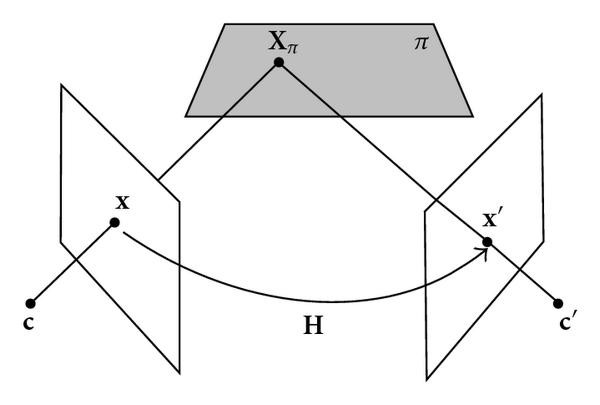
\includegraphics[width=15cm, height=6cm]{rette_epipolari}
	\caption{omografia per passare dal punto x a $x^{'}$}
\end{figure}





Per descrivere al meglio l'omografia si considera la figura 1 quindi

\begin{displaymath} 
	m^{'} = H_{\pi}* m. \iff m = P * M \iff M \in \Pi
\end{displaymath}


Possiamo considerare due tipologie di matrici di omografia, le omografie di rotazione e le omografie planari.
Per ottenere un omografia di rotazione si considerano le rette epipolari associate al punto M nella scena,
le matrici di proiezione completa delle due fotocamere sono le seguenti:

\begin{displaymath} 
	P = K[I|0]
\end{displaymath}


\begin{displaymath} 
	P^{'} = K^{'}[R|t]
\end{displaymath}

se applichiamo l'equazione delle rette epipolari in questo specifico caso otteniamo:


\begin{eqnarray}
	&m^{'} = H_{\pi} * m  \notag \\
	&= \lambda * K^{'} * R * K * m + K^{'}*t \notag
\end{eqnarray}

Questa omografia è anche chiamata omografia all'infinito perchè i punti sono collocati nella stessa posizione in entrambe le immagini a meno di una rotazione da applicare alle coordinate $(u,v)$ dell'immagine 1  per passare  alle coordinate dell'immagine 2 $(u',v')$.

la seconda tipologia di omografia  è chiamata omografia planare;
le considerazioni da fare in questo caso sono diverse,
dati due punti M e $M^{'}$,
Sia $M^{'}$ la rappresentazione di M nel riferimento della seconda  fotocamera $M^{'}$ = GM.
Si considera che 


\begin{eqnarray}
	&m^{'} = K^{'}\tilde{M}^{'} \label{eq:coord1} \\
	&m = K\tilde{M}
	\label{eq:coord2}
\end{eqnarray}

consideriamo anche la normale che è presente tra M e il piano,

\begin{align}
	n^{T}\tilde{M} = d \notag
\end{align}

svolgendo i calcoli si ottiene  :

\begin{eqnarray}
	& \tilde{M}^{'} = R\tilde{M} + t \notag \\
	\notag \\
	& n^{T}\tilde{M} = d \notag \\
	\notag \\
	& \frac{n^{T}\tilde{M}}{d} = 1 \notag \\
	\notag \\
	& \tilde{M}^{'} = R\tilde{M} + \frac{tn^{T}\tilde{M}}{d} \notag
\end{eqnarray}

la formulazione dell'omografia planare sostituendo a $\tilde{M}$ e $\tilde{M}^{'}$  i valori precedentemente definiti (\ref{eq:coord1},\ref{eq:coord2}),
otteniamo :


\begin{eqnarray}
	& K^{'  -1} m^{'} = (R+ \frac{tn^{t}}{d}) K^{-1}m \notag \\
	& m^{'} = K^{'}(R+ \frac{tn^{t}}{d}) K^{-1}m \notag \\
	& m^{'} = H_{\pi}m 
	\label{eq:hom}
\end{eqnarray}



Per il calcolo dell'omografia si considera l'equazione \ref{eq:hom}, quindi utilizzando il prodotto vettoriale tra $\tilde{m}$ e $H_{\pi}*m$,  si sfruttano le proprietà del prodotto di Kroneker  e si arriva alla formulazione 
\begin{align}
	\tilde{m} \times H_{\pi}*m = 0 \notag \\
	(m^{T} \otimes \tilde{m})*vect(H) = 0 \notag \\
	H \: = \: SVD(m^{T} \otimes \tilde{m})
\end{align}

per ottenere un numero sufficiente di equazioni servono quattro punti coniugati, perchè la matrice H ha 8 gradi di libertà e la coppia di punti $m^{T} \otimes \tilde{m}$ genera solo due equazioni linearmente indipendenti.














\section{Punti salienti}
I punti salienti in un immagine sono i punti che sono particolarmente individuabili e riconoscibili in un immagine.
Un punto saliente deve soddisfare delle caratteristiche:

\begin{itemize}
	\item \textbf{Scala} \\
	Un punto saliente deve essere invariante alla scala, cioè il punto deve essere riconoscibile in un immagine che lo
	inquadra ben visibilmente, sia in immagini più piccole in cui può essere descritto anche da pochi pixels
	\item \textbf{Luce} \\
	Anche in questo caso l'esposizione dell'oggetto a luci differenti non deve far cambiare la sua rilevazione
	\item \textbf{Orientamento} \\
	Possiamo considerare che un immagine possa essere acquisita da angolazioni differenti, in questo caso è
	necessario essere robusti alla rotazione della scena inquadrata


\end{itemize}



\subsection{Estrazione dei punti salienti}
Esistono diversi approcci per eseguire l'estrazione di punti salienti in un immagine, in questo caso si considera l'algoritmo SIFT,
ovvero ' Scale invariant feature transform'.




Il modello teorico di questo algoritmo utilizza il Laplaciano del filtro Gaussiano delle immagini, trovando quelli che sono punti di massimo o minimo, nell'implementazione pratica si utilizza 
la rappresentazione spazio-scala per rendere i punti salienti invarianti all'esposizione, ovvero si applicano alla stessa immagine filtri gaussiani con $\sigma$ differenti. 
Definiamo la rappresentazione spazio-scala come la funzione $L(x,y,\sigma)$, dove $\sigma$ è il valore che definisce la grandezza della distribuzione Gaussiana.

Nella rappresentazione spazio-scala si applica un filtro Gaussiano all'immagine, questo è un filtro di media particolare perchè se si applica un filtraggio con $\sigma$ molto piccolo si ottiene un immagine molto simile all'immagine di partenza,
se invece si applica un filtraggio con $\sigma$ grande, allora otterremo un immagine sfocata, questo perchè in base a $\sigma$ si
decide quanta importanza dare ai pixel adiacenti, ottenendo così un valore da sommare al pixel considerato quando si applica il filtraggio.
Con questo passaggio si ottiene l'invarianza all'esposizione della luce.

Attraverso le immagini piramidali invece si affronta e si risolve il problema legato alla scala, tramite questo approccio si calcolano i punti salienti di un immagine riducendo la dimensione dell'immagine,
quindi un punto saliente è tale se è possibile trovarlo in un range, solitamente su tre livelli, delle immagini che compongono la piramide.


Nell'implementazione di SIFT non si calcola direttamente il Laplaciano, ma le differenze delle immagini filtrate con kernel Gaussiano, in questo modo si ottengono dei punti di massimo e minimo che sono interpretati come punti salienti.


Se si combinano la rappresentazione scala-spazio e le immagini piramidali si ottengono dei punti salienti molto informativi perchè rispettano due dei tre requisiti;
un punto saliente è quindi un massimo o minimo locale che è presente in più livelli della piramide di immagini costruita iterativamente;
per risolvere il problema legato all'orientazione si utilizza il gradiente delle immagini che è invariante alla rotazione, quindi si utilizza come descrittore del punto un area  in cui si calcola il gradiente.
Il descrittore di un punto saliente è preso a partire da un intorno di $16 \times 16$ pixel in cui si calcola il gradiente, l'mplementazione del descrittore è effettuata tramite un vettore  colonna composto da 128 celle che descrivono l'orientamento del pixel adiacenti;
si sfrutta il descrittore quindi per eseguire il matching dei punti secondo un l'algoritmo che verrà introdotto e spiegato di seguito.



\subsection{Matching dei punti coniugati}
Una volta eseguita l'estrazione dei punti salienti è necessario mettere in relazione i punti delle due immagini considerate,
per svolgere questo compito importante si utilizza   un euristica basata sulla distanza tra i due punti considerati, quindi per ogni punto saliente della prima immagine si cerca il corrispettivo nella seconda immagine.\\
Si considera il caso in cui non tutti i punti salienti hanno un corrispettivo punto nella seconda immagine considerata, quindi si stabilisce una soglia sulla distanza calcolata tra i due punti per cui non si ottiene la corrispondenza, sarà quindi solo un sottoinsieme dei punti salienti a essere considerato.
Per eseguire il matching tra i punti si considera il descrittore del punto, se la distanza calcolata è sufficientemente bassa allora si considerano come coniugati, se sono presenti più punti che soddisfano questo vincolo allora si tiene il punto con minore distanza.

Pseudo codice dell'algoritmo di matching implementato in VlSift:

\begin{lstlisting}

matches = []
For each descriptor k1 in image 1:
    	closest_match_distance = inf
    	second_closest_match_distance = inf
	best_match = None
For each descriptor k2 in image 2:
      distance_squared = d(k1, k2)
      	if (distance_squared < closest_match_distance):
            	second_closest_match_distance = closest_match_distance
            	closest_match_distance = distance_squared
            	best_match = k2
    	If (threshold * closest_match_distance <
     		second_closest_match_distance AND best_match != None):
        		matches.Insert((k1,best_match, 
			closest_match_distance))
return matches

\end{lstlisting}


\section{Ransac}
Ransac è un algoritmo di statistica robusta che consente di eliminare gli outliers che non spiegano il modello fornito dai dati, nel caso considerato Ransac è utilizzato per migliorare il calcolo dell'omografia.

L'implementazione di questo algoritmo è descritta tramite i seguenti passaggi:

\begin{itemize}
	\item \textbf{input} \\
	In input si fornisce il set di dati che si vuole considerare, in questo caso un insieme di punti ricavati dal matching dei punti salienti eseguito da SIFT ($ConjugatePoints$), una soglia per l'errore ($\psi$) e il numero di iterazioni.
	\item \textbf{output} \\
	Come risultato si ottiene un sotto insieme dei punti forniti in input che rappresentano il modello, quindi sono gli Inliers.
	\item \textbf{Passo 1} \\
	Si scelgono casualmente due punti dal set dato come input.
	\item \textbf{Passo 2} \\
	Si calcola il valore $\tilde{\theta}$, che rappresenta la retta passante per i due punti scelti casualmente.
	\item \textbf{Passo 3} \\
	Si calcola consenso del modello rispetto ai dati : \\
	$\forall k \in{ConjugatePoints} $,\\
	$ y :  F(k,\tilde{\theta})< \psi$,\\ $y$ in questo passaggio rappresenta il set di punti che sono inliers, \\ F è la funzione che calcola la distanza euclidea tra retta e punto, se è inferiore a $\psi$ allora il numero di inliers aumenta.\\ $\psi$, (psi), è un numero che indica la tolleranza applicata alla distanza retta-punto, ad ogni ciclo confronto il numero massimo attuale di inlier con quello appena calcolato e mantengo solo quello con più inliers.
	\item \textbf{Passo 4} \\
	Si ripete 1-2-3 per il numero di iterazioni in input.
	\item \textbf{Passo 5} \\
	Fine dell'algoritmo, ritorno il set $y$ che ha il maggior numero di Inliers alla funzione principale che calcola l'omografia migliore.
	\item \textbf{Precisazione}\\
	$InliersConjugatePoints$ e $ConjugatePoints$ sono vettori colonna, e sono rappresentabili come $[X_{1},Y_{1},X_{2},Y_{2}]$; $(X_{1,i},Y_{1,i})$ è l'i-esimo punto saliente dell'immagine 1 e $(X_{2,i},Y_{2,i})$ è l'i-esimo punto saliente dell'immagine 2 coniugato all'i-esimo punto saliente dell'immagine 1.\\
	
	Nell'implementazione dell'algoritmo si analizzano con Ransac le variazioni dei punti salienti lungo gli assi X e Y,
	quindi ad esempio il primo set di punti considerato è $[Y_1,Y_2]$, inteso come i due vettori colonna dei punti salienti per l'asse Y.
	Si sceglie quindi il sotto insieme  più grande di punti che hanno una variazione simile tra le due immagini prese in considerazione (vedi esperimento 6).

\end{itemize}
\pagebreak
 Il risultato che si ottiene è mostrato nelle figure \ref{fig:corr_reg} e \ref{fig:wrong_reg}.
  Effettuando questa operazione è possibile eliminare tutti quei punti che statisticamente non hanno un corrispondente punto nella seconda immagine. Nel caso di studio preso in considerazione si ricerca la migliore omografia (H) per tentativi, questa è calcolata prendendo in modo casuale quattro punti dall'insieme di inliers forniti da Ransac ($InliersConjugatePoints$), appartenenti alle coppie derivanti dal matching effettuato sull’insieme di punti salienti, quindi si calcola l'omografia e si effettua la validazione sugli inliers ($InliersConjugatePoints$), la migliore omografia è quella con più inliers.
 
\begin{gather}
	ICP = InliersConjugatePoints \notag \\
	m  \in ICP \notag \\
	m = [m_1,m_2] , m_1 = [x,y,1] = [m_{1,i},m_{1,i},1]\notag \\
	K = H * m_1 \notag \\ 
	if  ( m_2 - K < \psi), \: then  \: inliers++  \notag
\end{gather}

Il risultato di questa fase è visibile tramite la figura \ref{fig:rgb_warp}.

	
\begin{figure}[H]
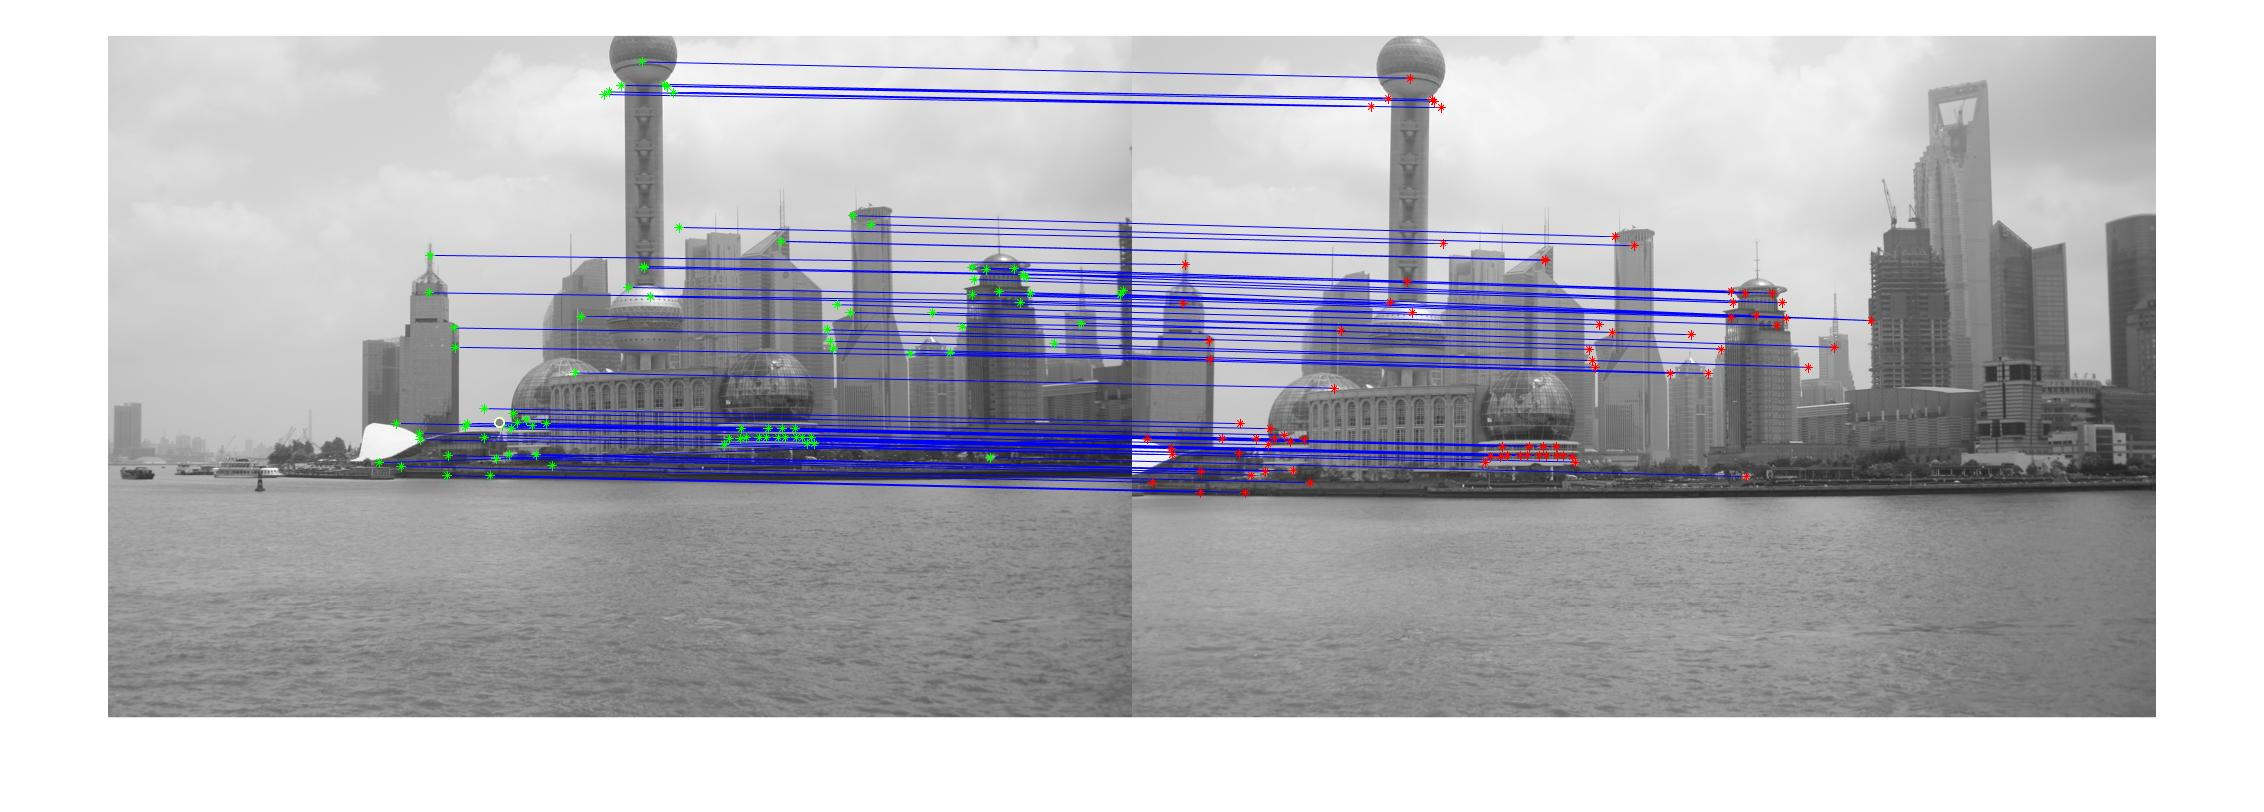
\includegraphics[width=\textwidth]{correct_match_salient_points.jpg}
\caption{Inliers risultanti da Ransac}
\label{fig:corr_reg}
\end{figure}

\begin{figure}[H]
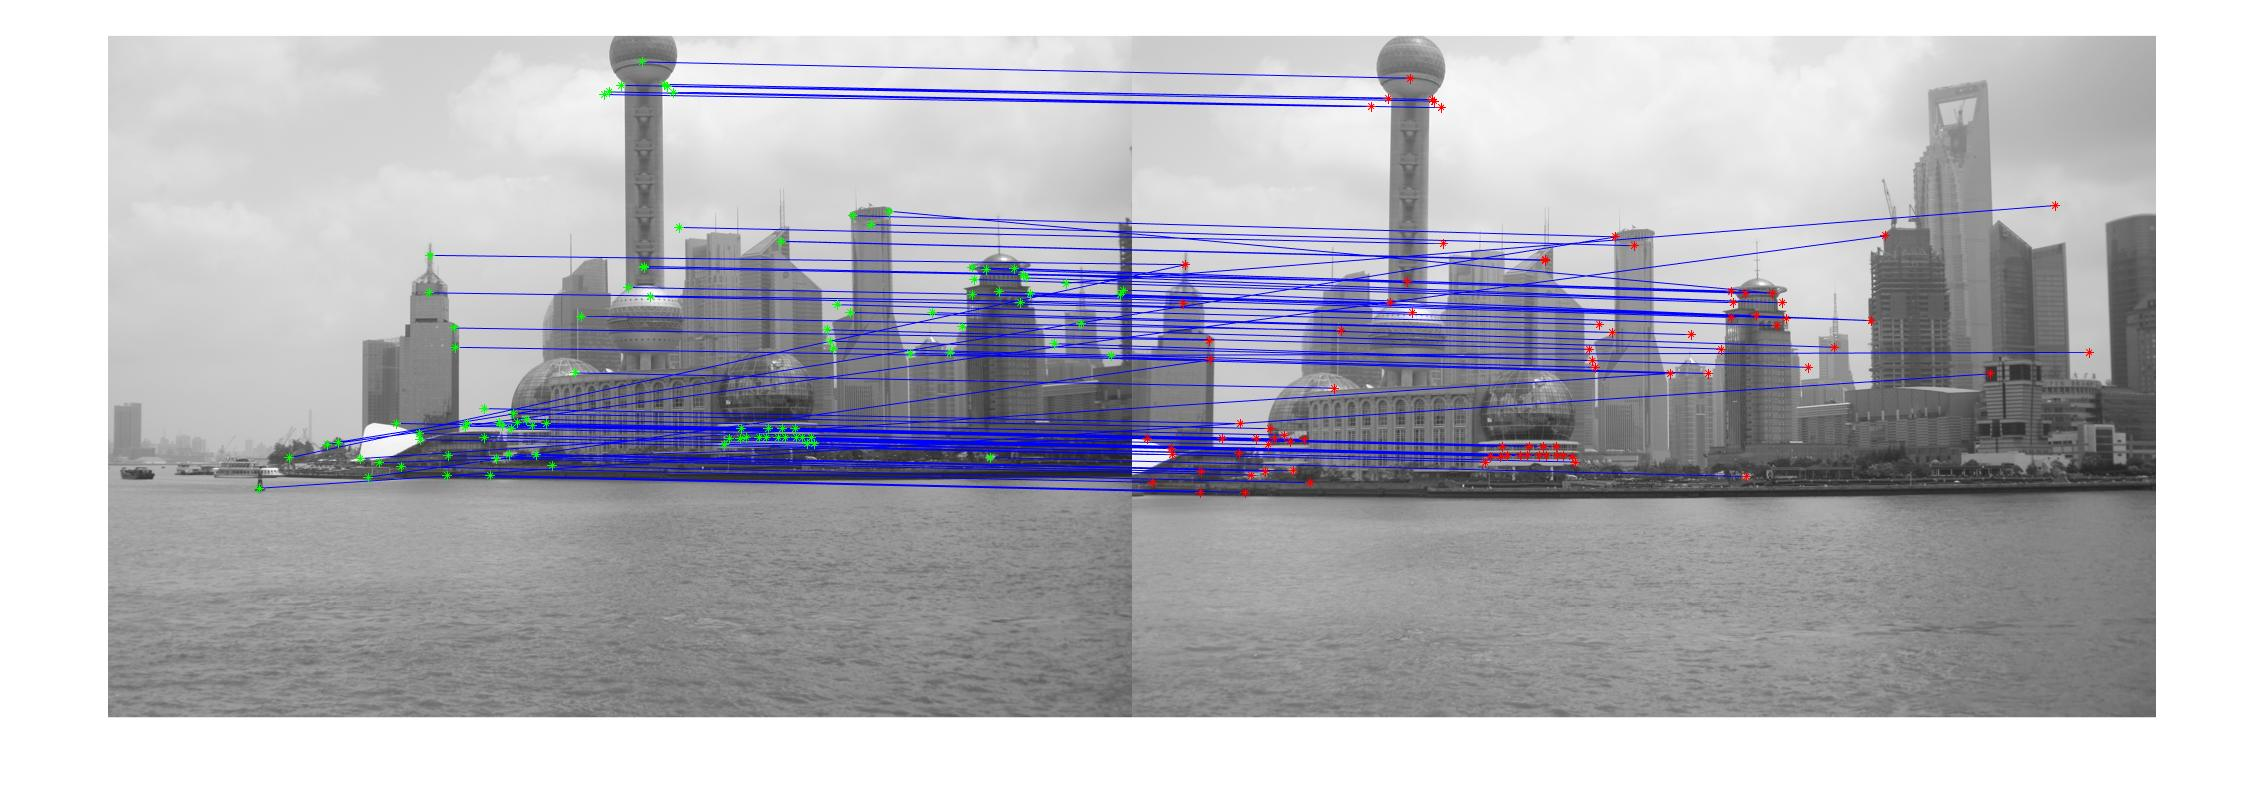
\includegraphics[width=\textwidth]{wrong_match_salient_points.jpg}
\caption{Punti salienti coniugati da SIFT}
\label{fig:wrong_reg}
\end{figure}



\begin{figure}[H]
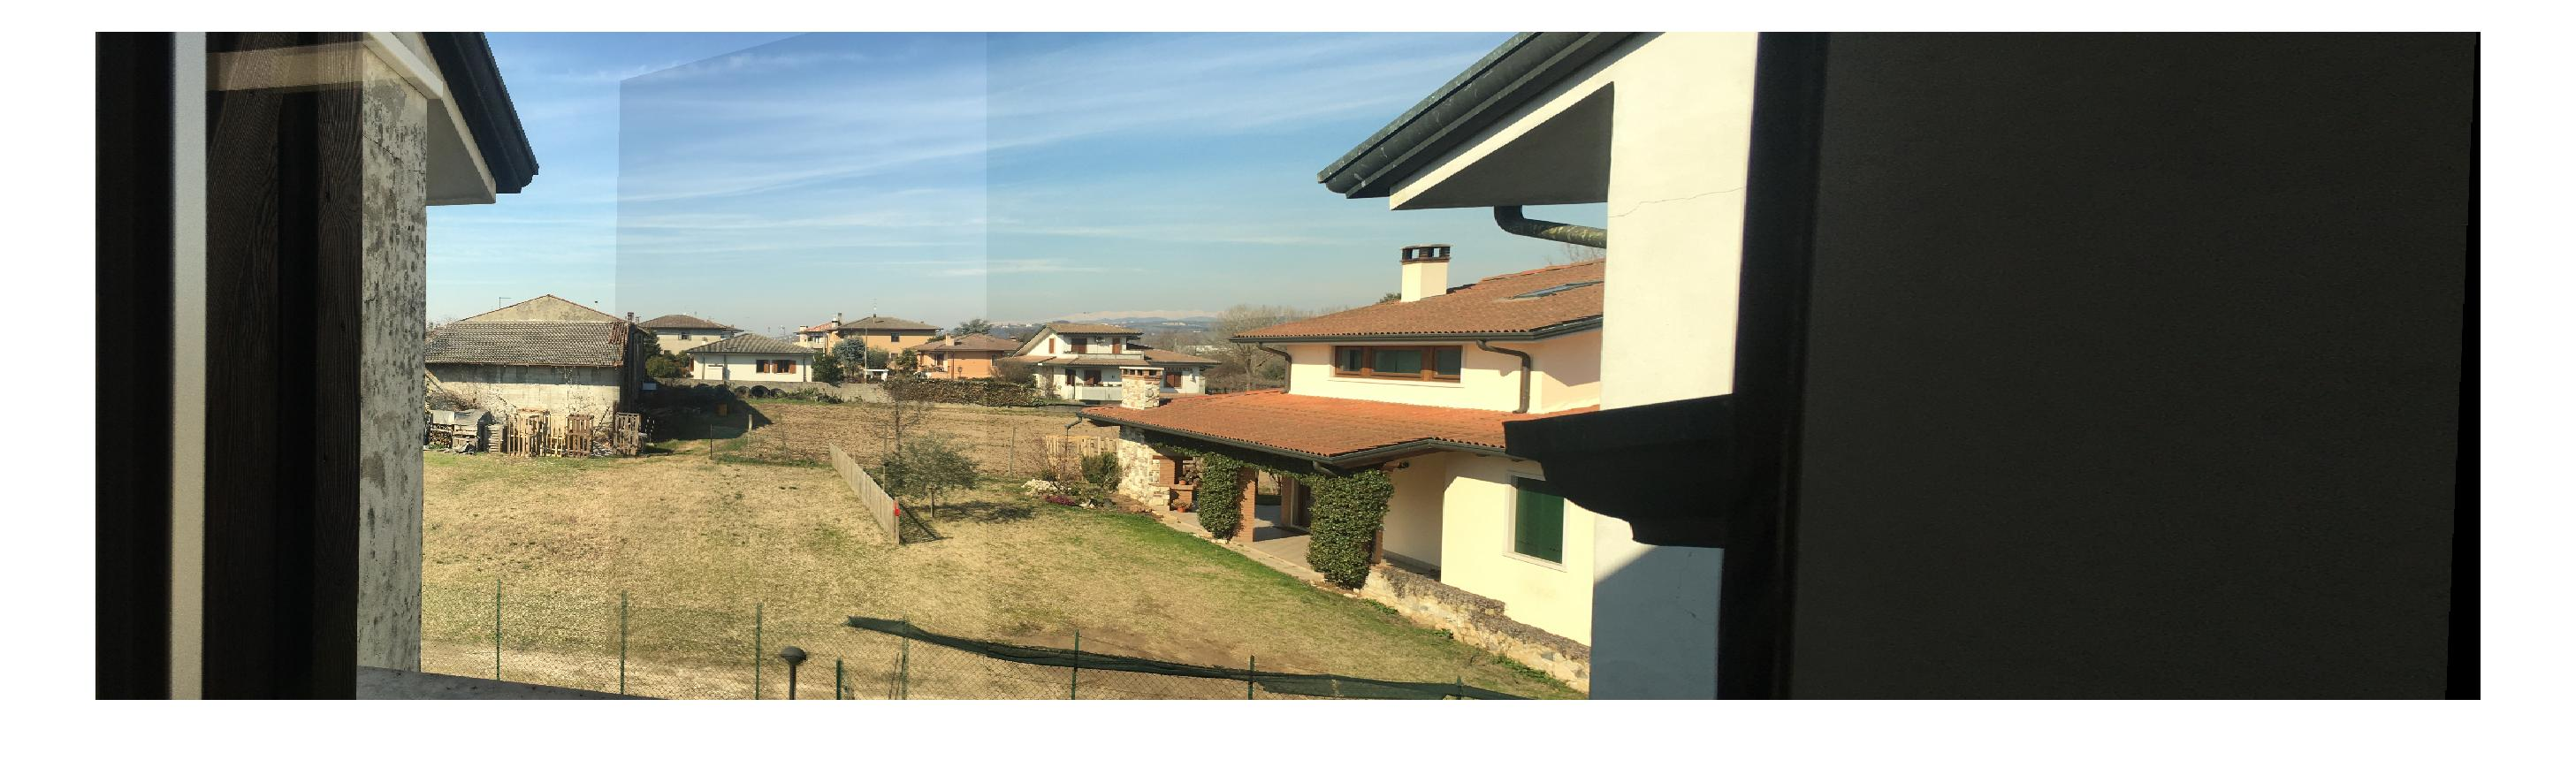
\includegraphics[width=\textwidth]{RGB_mosaicing}
\caption{Mosaicing con immagini RGB - Numero di foto : 2}
\label{fig:rgb_warp}
\end{figure}

\pagebreak

\section{Warping, Blending}
Il warping è un metodo che permette di modificare un immagine tramite un omografia,  l'azione di warping consiste nel calcolare la nuova posizione di ogni singolo pixel attraverso la matrice di omografia data in input.




\begin{figure}[H]
	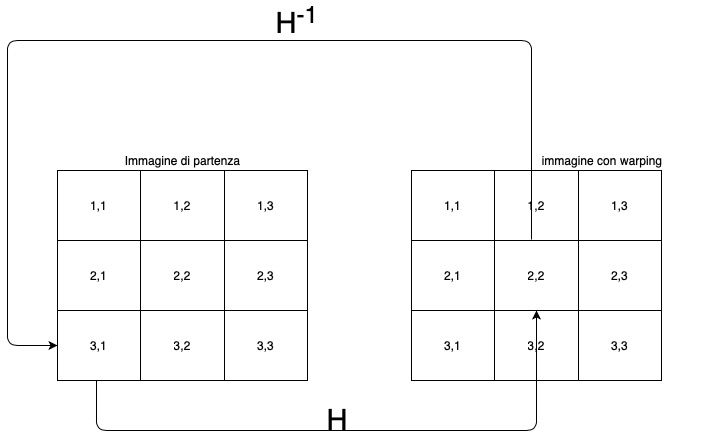
\includegraphics[width= \textwidth]{warping_schema.jpg}
	\caption{schema del warping diretto e indiretto}
	\label{fig:warp}
\end{figure}


Esistono due approcci ovvero diretto e indiretto, con l'approccio diretto si prende il pixel i-esimo dell'immagine di partenza e si calcola la sua nuova disposizione tramite la matrice di omografia nell'immagine di arrivo, nel metodo indiretto invece si esegue l'esatto opposto (vedi fig. \ref{fig:warp}).
Quando si applica un warping ad un'immagine è necessario tener conto di possibili stretching dei pixel o di compressione degli stessi perchè un singolo pixel dell'immagine di partenza può essere mappato in più pixel nell'immagine di arrivo e viceversa.
Nel programma sviluppato è stato inoltre incluso uno script per eseguire il Warping per immagini RGB, vedi fig \ref{fig:rgb_warp}.



Il blending consiste nell'unire due immagini, nel caso considerato la seconda immagine è l'immagine a cui è stato applicato un warping. Il warping tramite l'omografia permette di allineare le due immagini e quindi unirle.
Il problema principale del blending è l'uniformità del colore dell'immagine, per ottenere un buon risultato si calcola una maschera binaria che indica l'insieme di punti comuni tra le due immagini; ai punti comuni viene attribuito un valore che è la media tra i due presi dalle due immagini, i valori dei pixel non in comune vengono mantenuti dalle immagini di partenza.

Per quanto riguarda la gestione degli angoli ho utilizzato una funzione apposita da me creata chiamata  $"createMask"$, la funzione genera una maschera a partire da un concetto semplice, quando si effettua il Warping e il Blending l'immagine risultante ha un bordo nero che la circonda, che può essere più o meno grande, quindi creo la maschera esattamente grande quanto l'immagine e inizializzo tutti i valori al massimo (255), quindi creo un indice che segna la posizione di ogni singolo pixel inferiore ad una soglia, l'indice fa riferimento ai valori dei pixel dell'immagine, ho scelto 1 come soglia, assegnando a quel punto il valore zero nella maschera; infine effettuo la binarizzazione della maschera e attraverso una seconda funzione, riduco il più possibile i bordi neri introdotti dal Warping e Blending utilizzando la maschera.



\section{Risultati e conclusioni}

Tutti i panorama di seguito mostrati sono stati creati a partire da quattro o più immagini che descrivono la scena.
L'algoritmo implementato segue una pipeline che è la seguente:
\begin{figure}[H]

\includegraphics[width=\textwidth]{pipeline}
\end{figure}

I parametri a scelta dell'utilizzatore sono:
\begin{itemize}
	\item \textbf{Soglia per i punti salienti} \\
	Se si fornisce una soglia alta verranno considerati solo i punti più significativi e di conseguenza i punti salienti saranno un insieme molto più piccolo rispetto a un valore di k più piccolo
	\item \textbf{Numero di iterazioni Ransac} \\
	Il numero di iterazioni influisce direttamente sulla qualità dell'omografia e sul tempo  impiegato per arrivare al risultato finale
	\item \textbf{Tolleranza punti coniugati (psi)}\\
        Questo parametro rappresenta la tolleranza che si applica nel calcolo dei punti di corrispondenza, se il punto si trova entro N pixel, come da parametro, lo si considera valido
\end{itemize}

I risultati in questo caso dipendono molto dalla bontà della scena ripresa, in questo caso si sono state utilizzate immagini campione derivanti da un database di ADOBE, il pacchetto si chiama $"adobe-panoramas"$, in questo database sono state scelte solo alcuni dei panorama, perchè non tutti i set non rispettano i vincoli imposti dal problema considerato.


\subsection{Esperimento 1 :}



Nel primo esperimento ho preso in considerazione un set di foto che rappresentano un panorama di una montagna, questo è il caso che mette maggiormente in difficoltà l'algoritmo perchè si considerano molte foto, quindi il rumore che viene introdotto ad ogni ciclo viene sempre più amplificato a causa del warping e peggiora la qualità finale della mosaicatura.

Dettagli dell'esperimento:
\begin{itemize}
	\item \textbf{Numero di foto :} \\
	10 foto 1024 x 683 pixel
	\item \textbf{Numero di iterazioni Ransac : } \\
	1000 iterazioni
	\item \textbf{Tolleranza punti coniugati (psi) :}\\
        1 pixel 
        \item \textbf{Considerazioni : }\\
        in questo caso il risultato è buono, si notano delle porzioni non correttamente allineate nell'immagine, se si prendono in esame meno fotografie il risultato è migliore.
        
\end{itemize}


\begin{figure}[H]
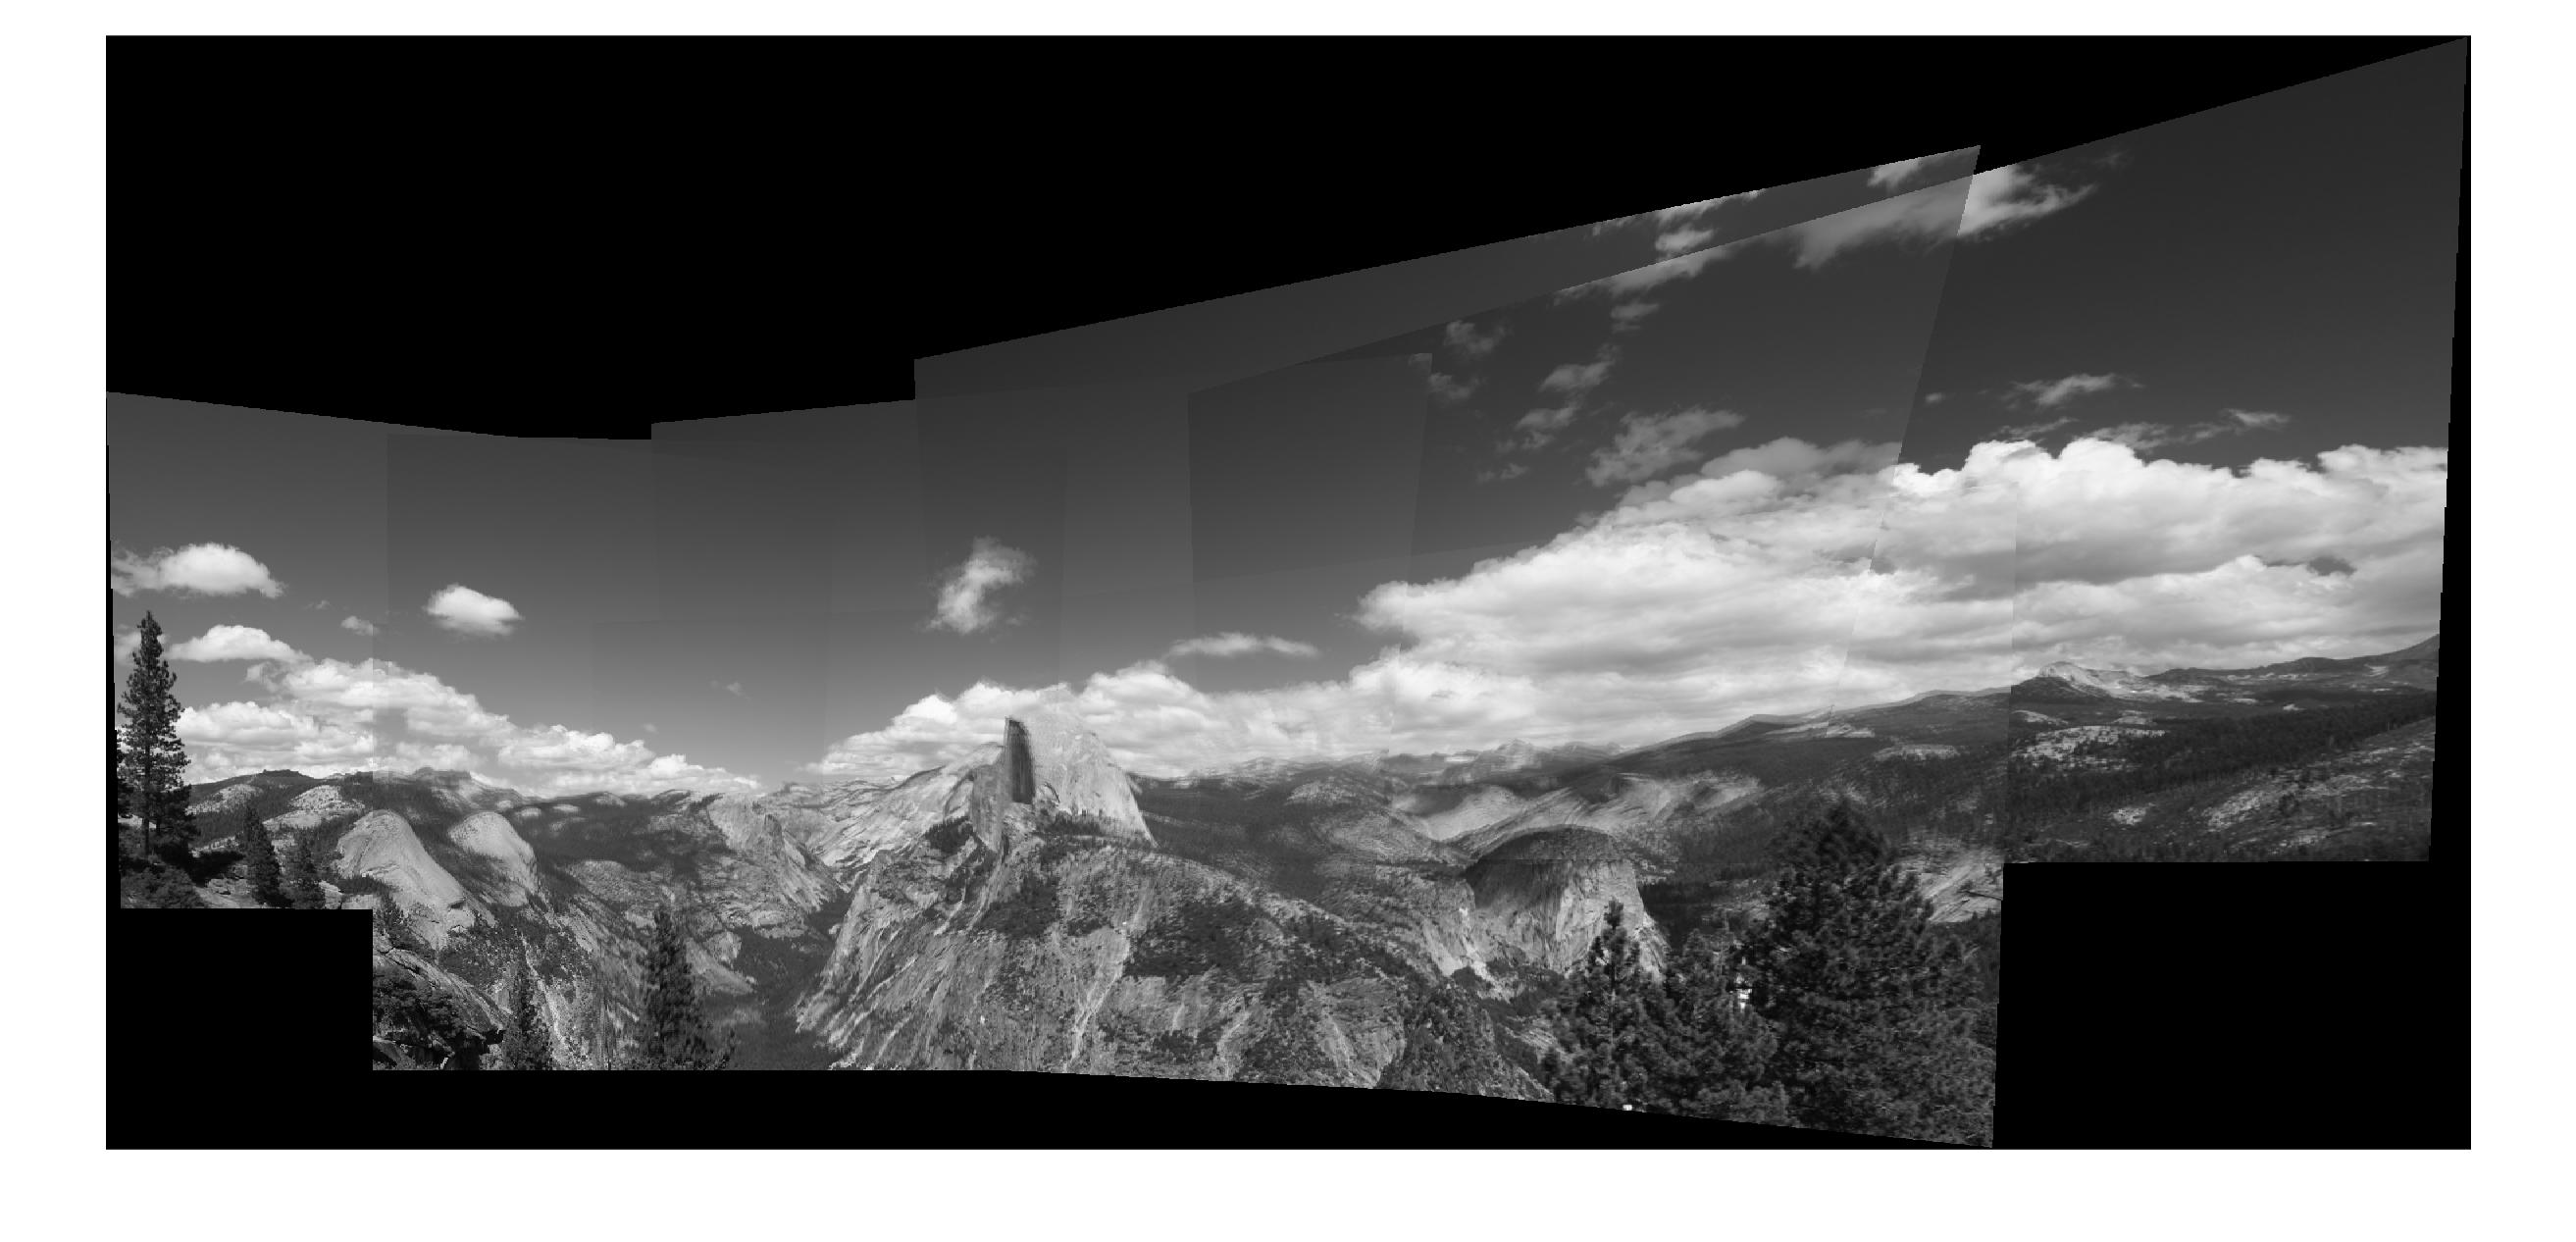
\includegraphics[width=\textwidth]{montagna_14_foto.jpg}
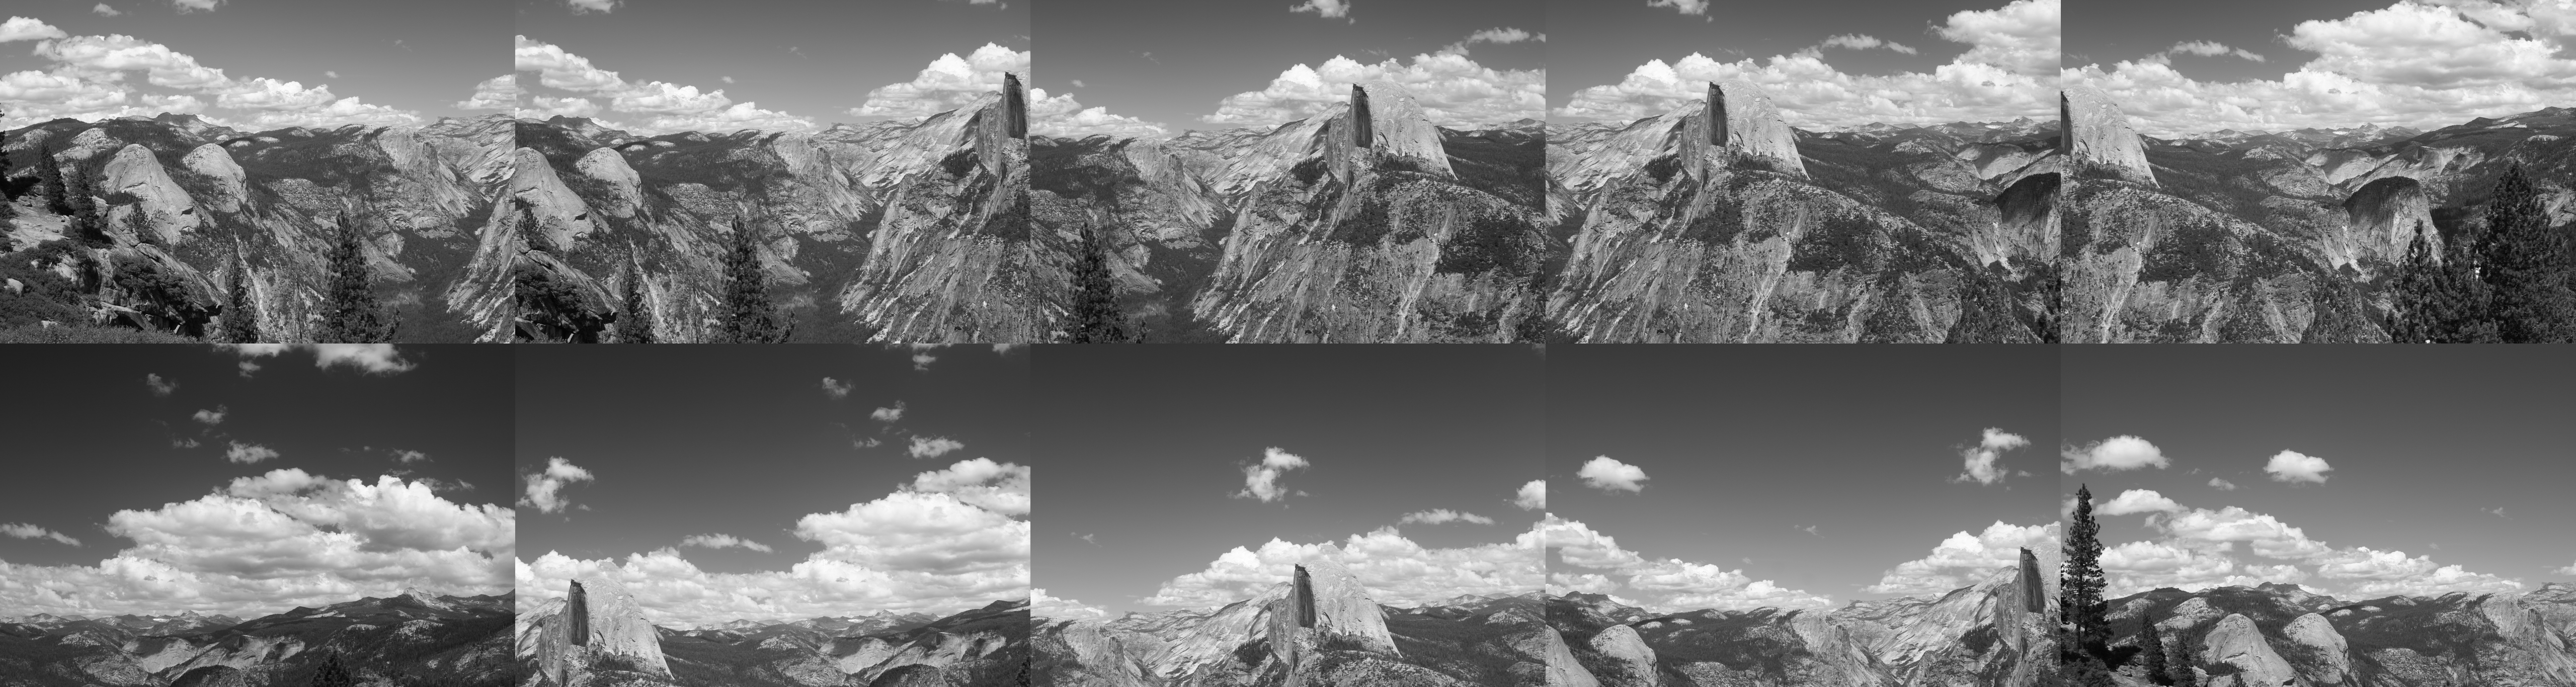
\includegraphics[width=\textwidth]{foto_mosaico_montagna.png}

\caption{Mosaicatura e set di immagini iniziali}
\end{figure}


\subsection{Esperimento 2 :}
In questo esperimento prendo in considerazione una quantità inferiore di fotografie ritraenti lo stesso panorama, ma con una tolleranza maggiore dei punti coniugati nella scelta dell'omografia migliore.
Dettagli dell'esperimento:
\begin{itemize}
	\item \textbf{Numero di foto :} \\
	4 foto 1024 x 683 pixel
	\item \textbf{Numero di iterazioni Ransac : } \\
	1000 iterazioni
	\item \textbf{Tolleranza punti coniugati (psi) :}\\
        5 pixel
        \item \textbf{Considerazioni : }\\
        in questo caso il risultato è migliore rispetto al precedente perchè si considerano meno fotografie, quindi la distorsione introdotta dal warping è minore, si sottolinea il fatto che la tolleranza in questo caso è di 5 pixel, quindi esiste una correlazione tra numero di foto e tolleranza dei punti coniugati.
        
\end{itemize}


\begin{figure}[H]
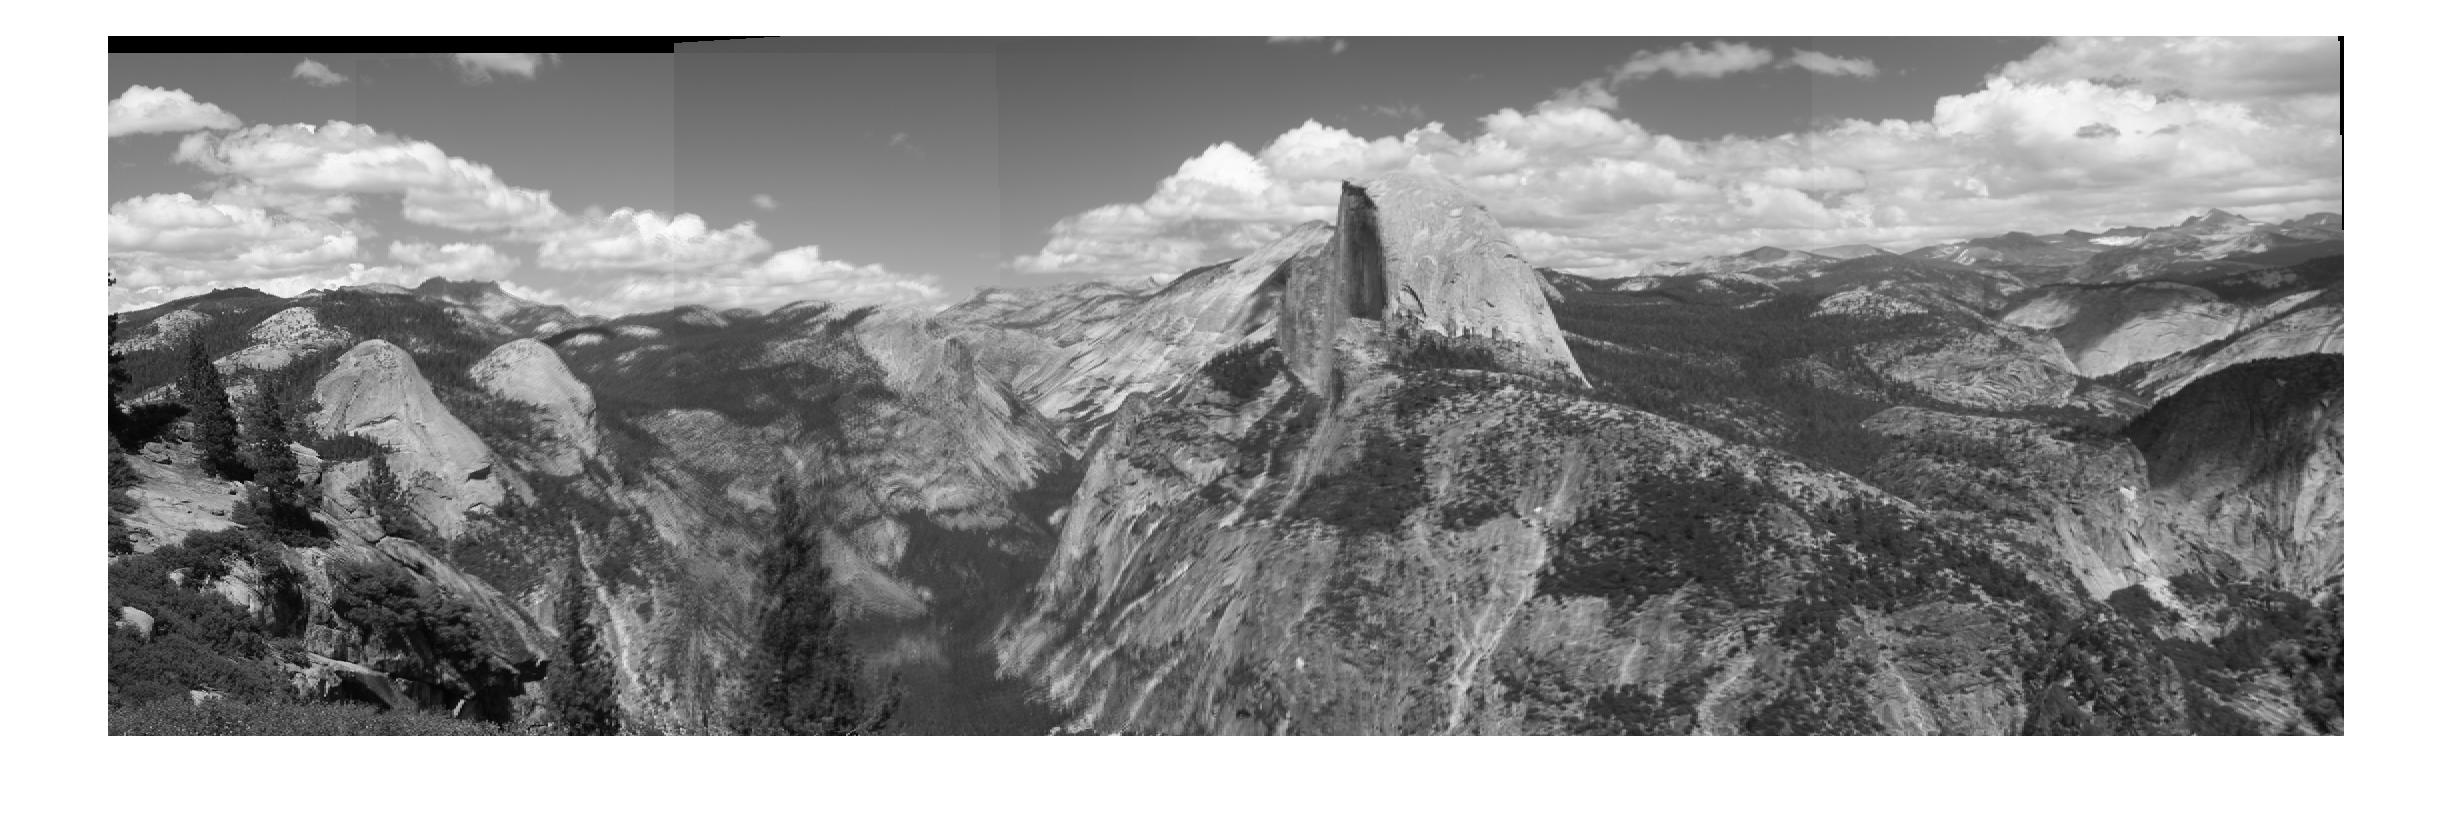
\includegraphics[width=\textwidth]{montagna_psi_5.jpg}
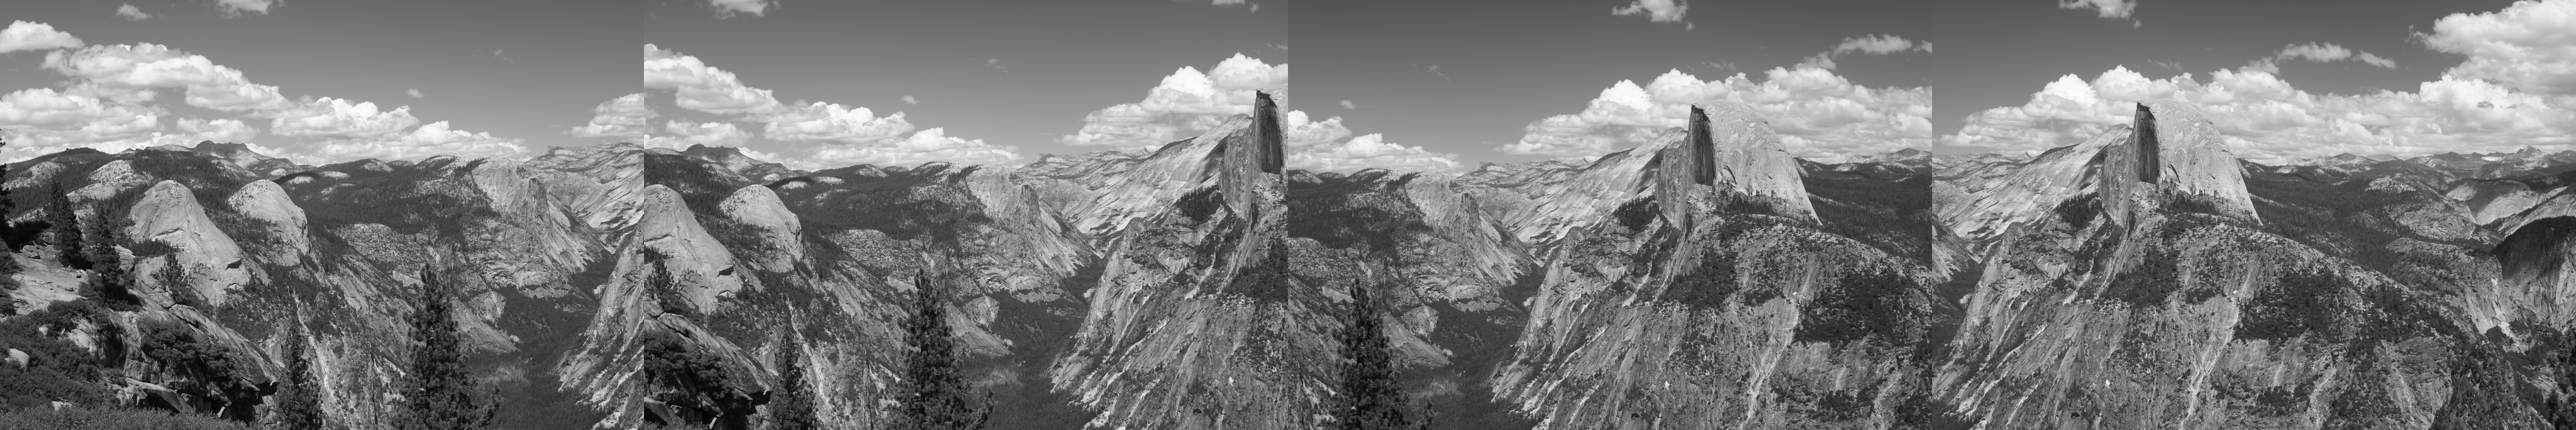
\includegraphics[width=\textwidth]{foto_mosaico_montagna2.png}

\caption{Mosaicatura e set di immagini iniziali}
\end{figure}


\subsection{Esperimento 3 :}
In questo esperimento invece  ho cercato di validare l'utilità di Ransac, quindi ho eliminato la parte in cui si eliminano gli outliers dall'insieme di punti coniugati forniti da SIFT.
Dettagli dell'esperimento:
\begin{itemize}
	\item \textbf{Numero di foto :} \\
	2 foto 1024 x 683 pixel
	\item \textbf{Numero di iterazioni Ransac : } \\
	Non utilizzato
	\item \textbf{Tolleranza punti coniugati (psi) :}\\
        1 pixel
        \item \textbf{Considerazioni : }\\
        in questo caso il risultato è nettamente peggiore rispetto ai due precedenti, non è stato possibile andare oltre due fotografie perchè il disallineamento è eccessivo.        
\end{itemize}


\begin{figure}[H]
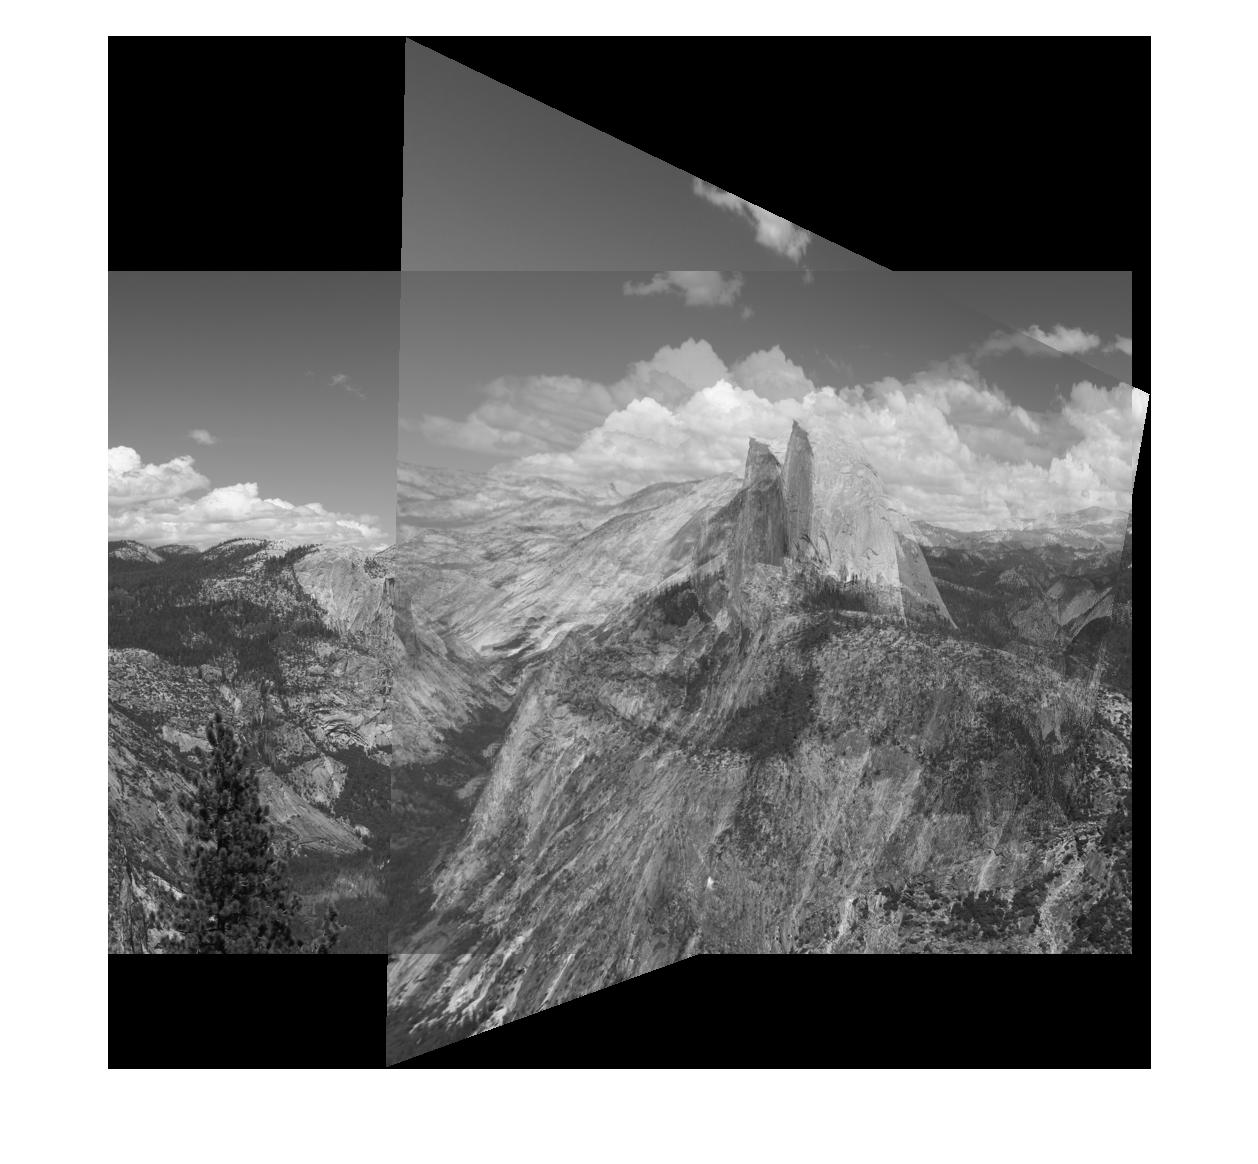
\includegraphics[width=\textwidth]{only_sift.jpg}
\caption{Mosaicatura con solo SIFT}
\end{figure}




\subsection{Esperimento 4 :}
In questo esperimento ho voluto validare anche l'importanza del margine di tolleranza (psi), e allo stesso tempo cercando un valore ragionevole per ottenere una mosaicatura corretta.
Dettagli dell'esperimento:
\begin{itemize}
	\item \textbf{Numero di foto :} \\
	4 foto 1024 x 683 pixel
	\item \textbf{Numero di iterazioni Ransac : } \\
	1000 iterazioni
	\item \textbf{Tolleranza punti coniugati (psi) :}\\
        25 pixel
        \item \textbf{Considerazioni : }\\
        in questo caso il risultato è peggiore perchè il rumore introdotto da una tolleranza di 25 pixel è eccessivo nel calcolo dell'omografia migliore, quindi l'immagine presenta evidenti errori di allineamento e risulta distorta.
\end{itemize}


\begin{figure}[H]
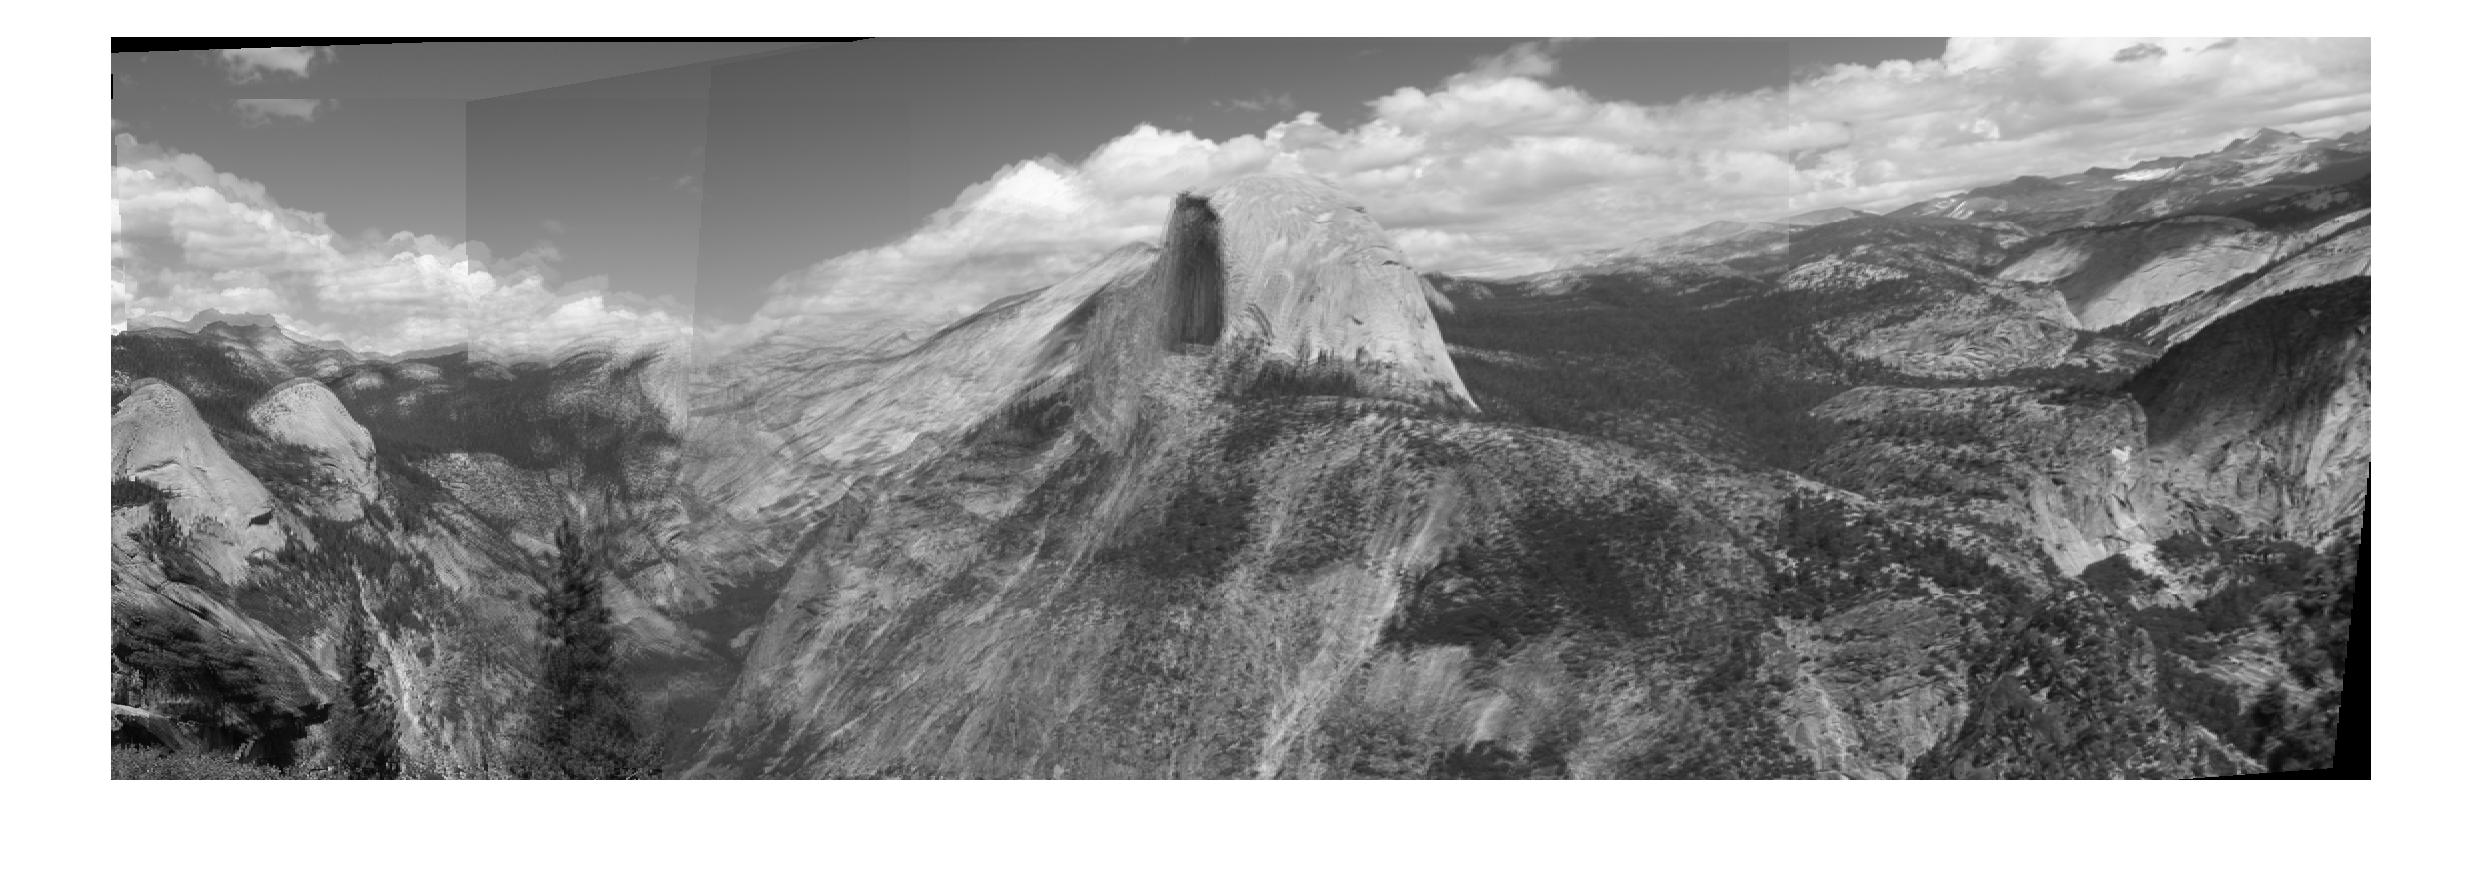
\includegraphics[width=\textwidth]{montagna_psi_25.jpg}
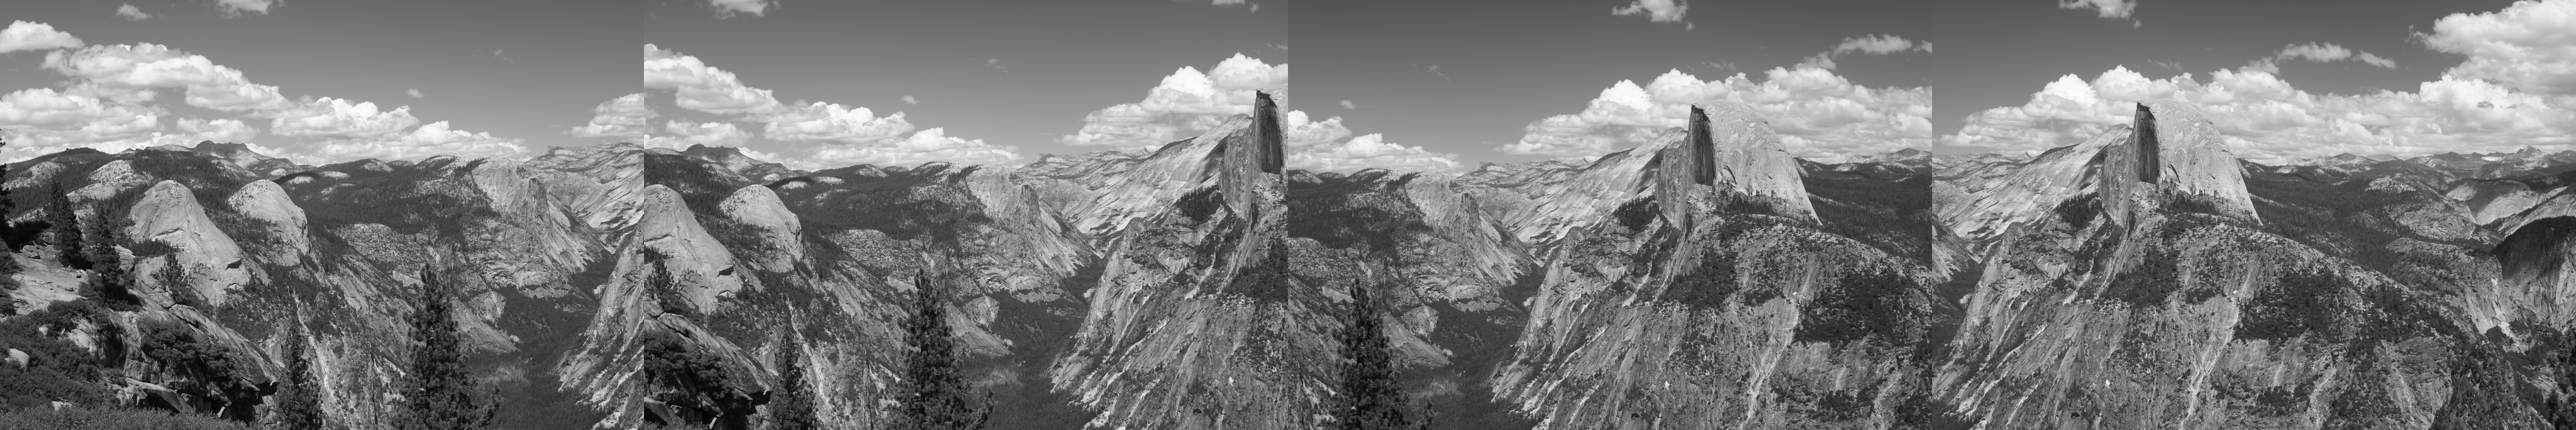
\includegraphics[width=\textwidth]{foto_mosaico_montagna2.png}
\caption{Mosaicatura e set di immagini iniziali}
\end{figure}


\subsection{Esperimento 5 :}
In questo esperimento invece prendo in considerazione un panorama differente per testare l'effettiva applicabilità dell'algoritmo anche ad altre tipologie di panorama. In questo caso ho preso il panorama di una via di Rio de Janeiro.
Dettagli dell'esperimento:
\begin{itemize}
	\item \textbf{Numero di foto :} \\
	8 foto 1024 x 768 pixel
	\item \textbf{Numero di iterazioni Ransac : } \\
	1000 iterazioni
	\item \textbf{Tolleranza punti coniugati (psi) :}\\
        1 pixel
        \item \textbf{Considerazioni : }\\
        in questo caso il risultato è ottimo, la mosaicatura non presenta distorsioni evidenti, tranne per un ramo nella parte superiore centrale dell'immagine.
\end{itemize}


\begin{figure}[H]
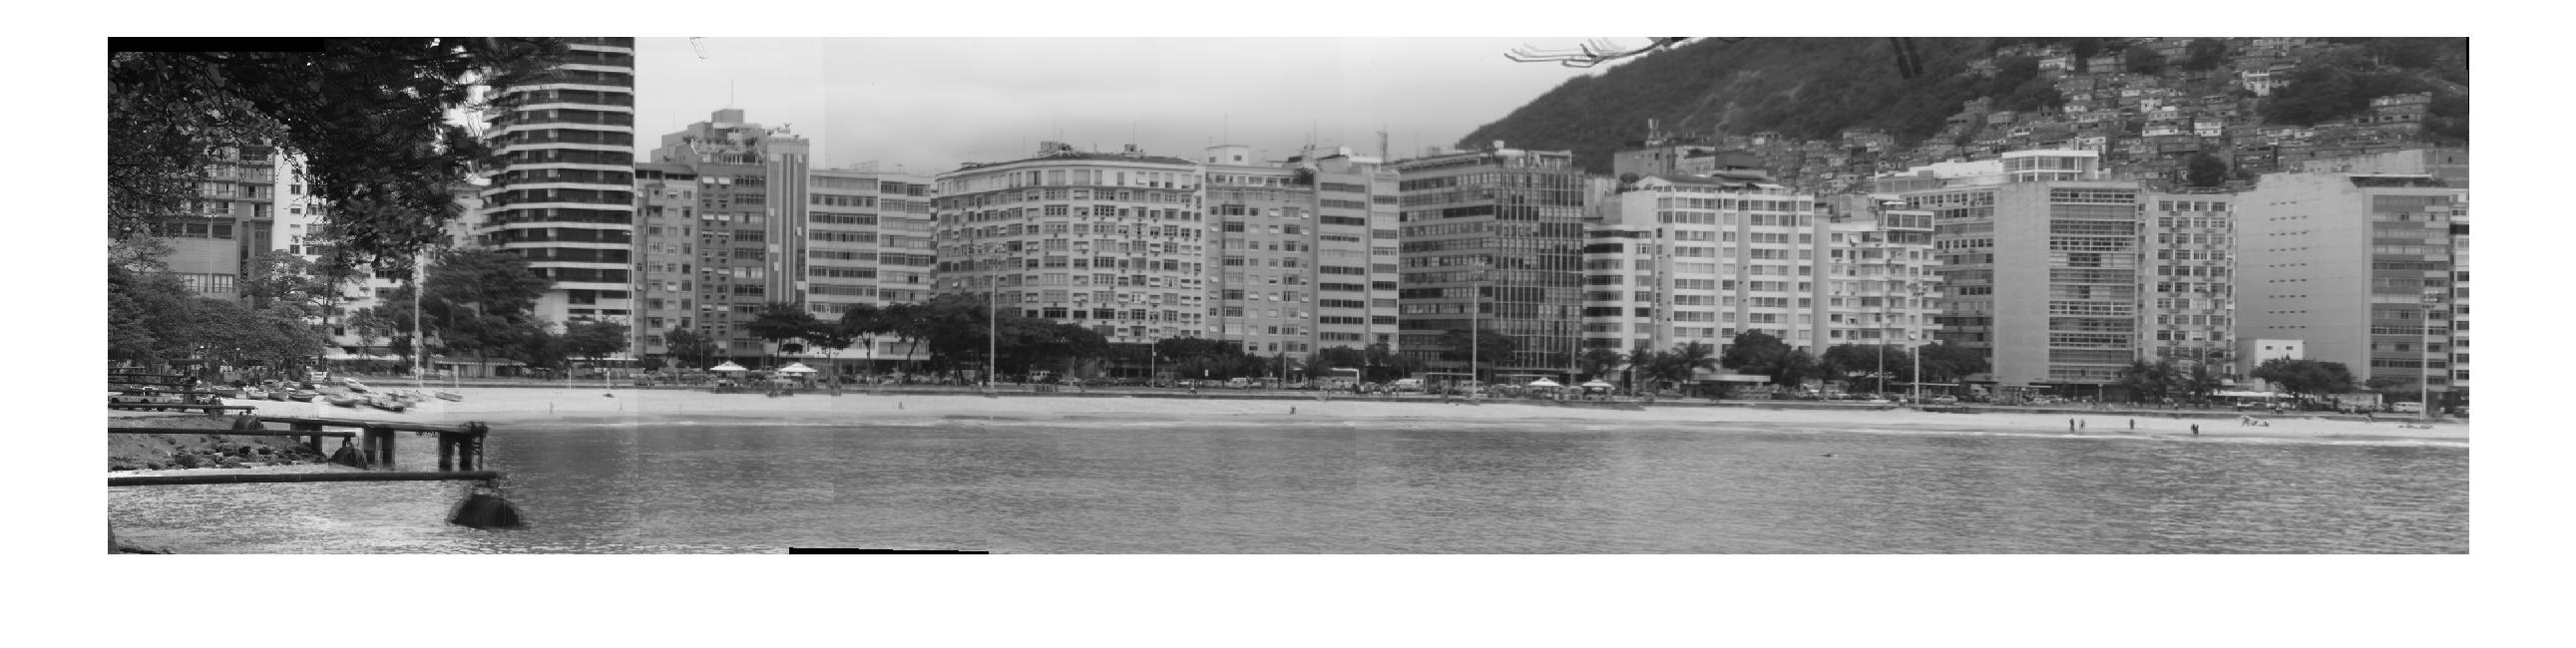
\includegraphics[width=\textwidth]{rio.jpg}
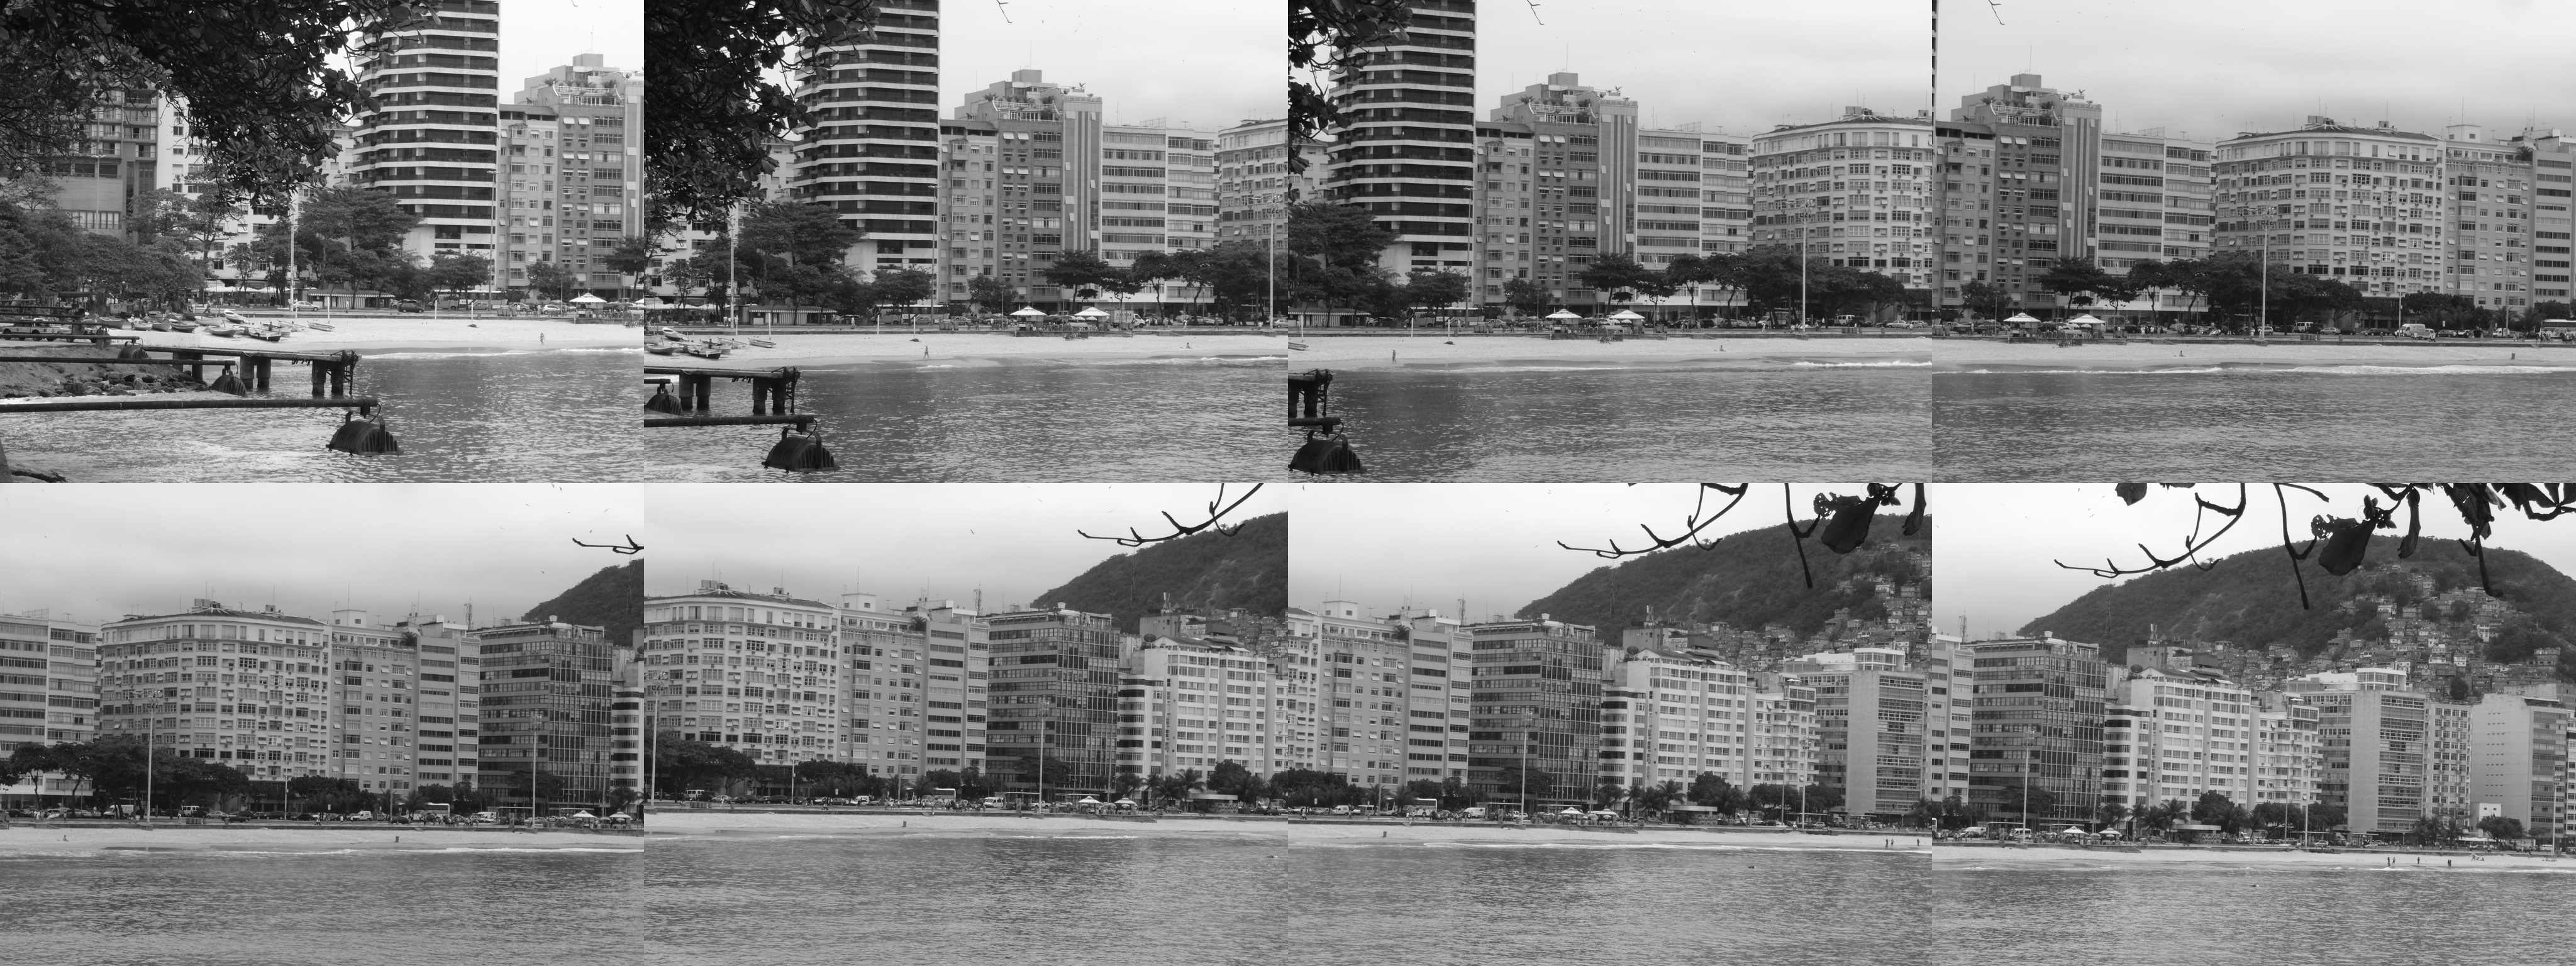
\includegraphics[width=\textwidth]{foto_mosaico_rio.png}
\caption{Mosaicatura e set di immagini iniziali}
\end{figure}




\subsection{Esperimento 6 :}

Per rendere evidente l'effettiva utilità di Ransac ho incluso un immagine in cui è ben visibile  il funzionamento di Ransac, l'insieme di punti deriva dall'insieme dei punti messi in relazione da SIFT, in particolare si confronta l'andamento dei punti coniugati lungo l'asse delle ordinate e poi delle ascisse.


L'insieme di punti rappresentati sono i punti normalizzati ricavati dal matching di SIFT, in verde sono evidenziati gli Inliers.

\begin{figure}[H]
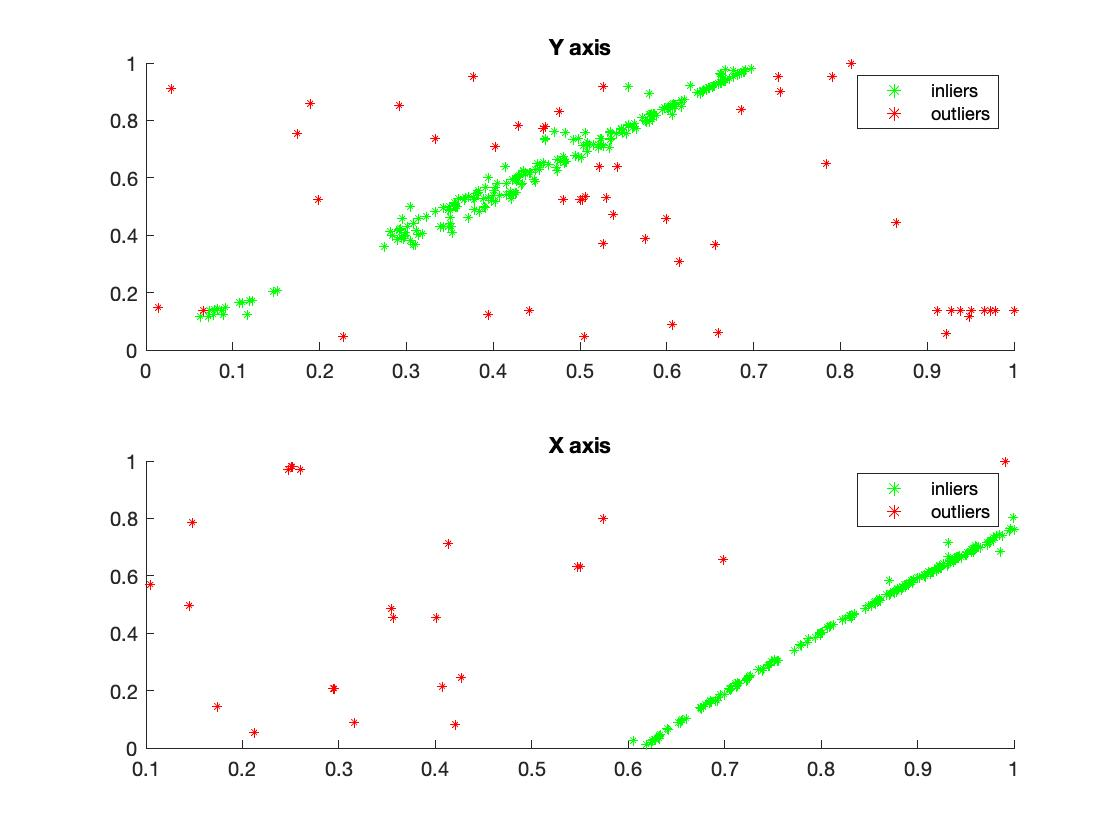
\includegraphics[width=\textwidth]{rio_out_inliers_ultima_iterazione.jpg}
\caption{Applicazione di Ransac - Set punti coniugati ottenuti da SIFT }
\label{fig:ransac_schematic}
\end{figure}

Possiamo vedere nella figura \ref{fig:ransac_schematic}, che viene trovato un modello tra tutti i punti che sono stati coniugati, tra questi sono presenti coppie di punti che non sono corretti, questo è possibile verificarlo nella seguente immagine che valida l'importanza di Ransac.


\begin{figure}[H]
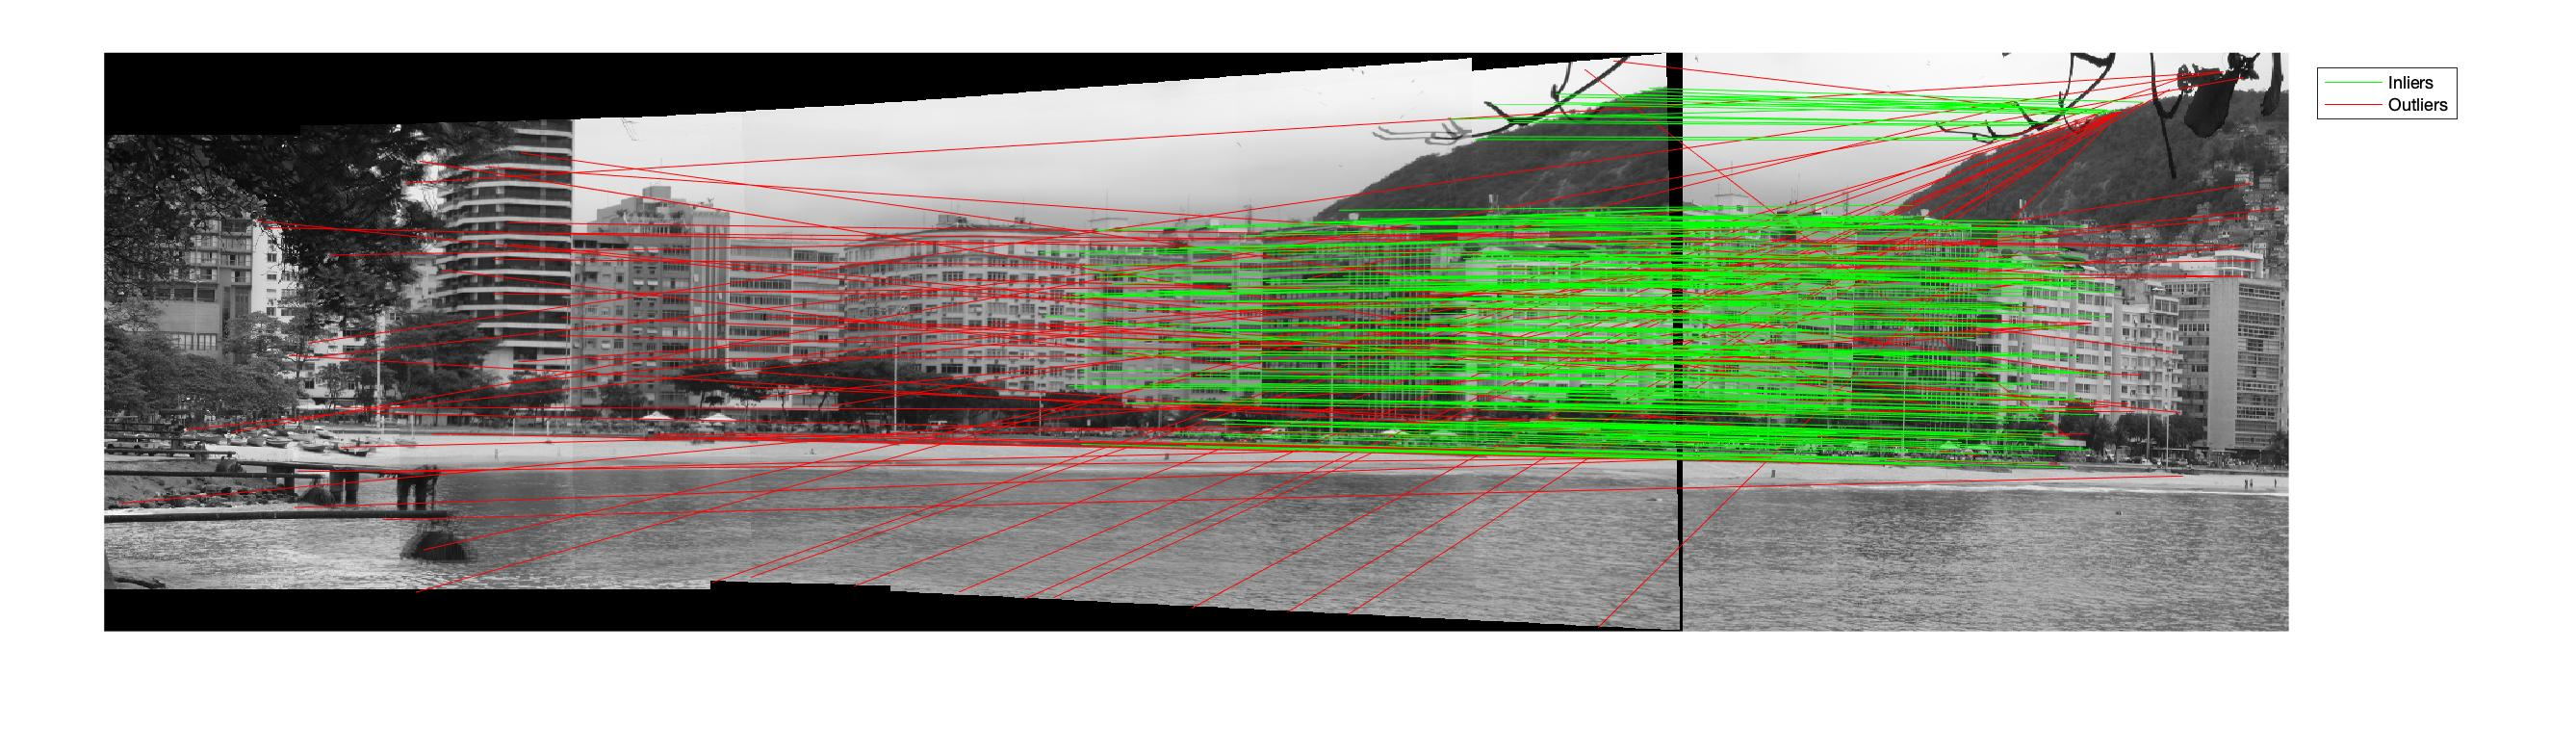
\includegraphics[width=\textwidth]{rio_check_ransac_immagine_ultima_iterazione.jpg}
\caption{Applicazione di Ransac - Rio de Janeiro}
\label{fig:ransac}
\end{figure}

\subsection{Considerazioni finali}

L'algoritmo funziona correttamente se si imposta una soglia bassa per la tolleranza dei punti coniugati, se si considera un intorno superiore ai 5 pixel è possibile ottenere immagini con molto rumore o immagini distorte.
Si fa notare che per le immagini prese in considerazione il valore massimo di PSI per ottenere un buon risultato è esattamente 
5, per valori superiori l'immagine finale risulta eccessivamente distorta, solo per una scena è stato possibile superare questo limite ed ottenere comunque una ricostruzione non eccessivamente distorta, vedi esperimento 2.
Per testare l'effettiva utilità di Ransac nel calcolo dell'omografia, è stato eseguito un test in cui si toglie la parte di ottimizzazione effettuata da Ransac nell'individuare la migliore omografia, il risultato è evidente infatti in tutti i casi non è stato possibile trovare un'omografia corretta; l'unico modo per trovare con solo SIFT un'omografia corretta è impostare una soglia molto alta per i punti salienti, altrimenti la probabilità di trovare punti salienti migliori diminuisce, in ogni caso è molto difficile trovare una corretta omografia considerando solo i punti salienti coniugati derivanti da SIFT, vedi esperimento 3.



Da questi dati emerge chiaramente il vantaggio dell'applicazione di una tecnica di statistica robusta come Ransac in problemi che riguardano il matching tra punti salienti, nel caso dell'utilizzo del solo matching tra punti salienti non è stato possibile trovare un omografia soddisfacente, invece tramite Ransac è stato possibile trovare un omografia corretta e unire tutte le immagini che riprendono una scena planare senza introdurre una distorsione o rumore eccessivo nell'immagine finale che inquadra l'intero panorama. 









\end{document}  